% LaTeX source for textbook ``Think C++, a game perspective''
% Copyright (C) 2023  Lisa Patacchiola, Allen B. Downey


\DocumentMetadata{}
\documentclass{book}
\usepackage[pdftex,
            pdfauthor={Lisa Patacchiola and Allen B Downey},
            pdftitle={ThinkCPP, a game perspective},
            pdfsubject={Programming},
            pdfkeywords={c++, programming, games},
            pdfproducer={Latex with hyperref, or other system},
            pdfcreator={pdflatex, or other tool}]{hyperref}
\usepackage{makeidx}
\usepackage{url}
\usepackage{listings}
\usepackage{graphicx}
\graphicspath{ {./images/} }
\pssilent
%\usepackage[tagged, highstructure]{accessibility}
%\usepackage{tagpdf}
\usepackage{color}
\definecolor{dkgreen}{RGB}{46,133,64}
\definecolor{gray}{rgb}{0.5,0.5,0.5}
\definecolor{mauve}{rgb}{0.58,0,0.82}
\definecolor{lightblue}{rgb}{0.5, 0.6, 0.8}
\lstset{language=[ANSI]C++,
keywordstyle=\color{blue}\bfseries, % style for keywords
showstringspaces=false,
   commentstyle=\color{dkgreen},
   stringstyle=\color{mauve},
   basicstyle={\small\ttfamily},
  % backgroundcolor=\color{lightblue}
}   
%\renewcommand\cftsecnumwidth{2em}

\title{Think C++, a game perspective}

\author{Lisa Patacchiola, Allen B. Downey (original author)}
\date{3/15/2023}

\sloppy
\setlength{\topmargin}{0.75in}
\setlength{\headsep}{0.5in}
\setlength{\oddsidemargin}{1.0in}
\setlength{\evensidemargin}{.95in}
\makeindex

\begin{document}

\title {Think C++, a game perspective}
\date {Version 2.0 alpha 0.6}
\maketitle

\vspace{2in}
\begin{center}
{\Large Think C++, a game perspective}

\vspace{0.25in}

Copyright (C) 2023 Lisa Patacchiola and Allen B. Downey
\end{center}
\vspace{0.25in}

Permission is granted to copy, distribute, transmit and adapt this
work under the Creative Commons Attribution-NonCommercial-ShareAlike 4.0
International License: \url{https://creativecommons.org/licenses/by-nc/4.0/}.

If you are interested in distributing a commercial version of this
work, please contact the author.

\bigskip
The \LaTeX\ source and code for this version of the book are available from

\bigskip
\url{https://github.com/lpatacch/thinkCPPGames}

\bigskip
The \LaTeX\ source and code for the original book is available from

\bigskip
\url{https://github.com/AllenDowney/ThinkCPP}



\frontmatter
% LaTeX source for textbook ``Think C++, a game perspective''
% Copyright (C) 2023  Lisa Patacchiola

\chapter{Preface}

\section{Notes from Lisa}
Hi! If you are reading this note, you are reading an alpha version of this book. That means that I have not completely converted the book over the the format I eventually want to have. Double check my github account that you have the most recent version.

If this is the most recent version, here is the information so far.

Chapter 1 and 2 has some work done. I have changed some of the examples to have more of a game flavor. I have moved Functions a bit further back in the book and have moved If statements up to Chapter 3. I have also brought switch statements up as well. Chapter 3 has been started, but has not been converted over yet. You will still find "FIXME"s in the chapter, and I have not switched the examples to something more game-like. I have put stubs for flowcharts and pseudo code, but I have not put anything in there yet. Other chapters have had small changes, mostly so the previous links are no longer broken.

I have added an appendix to talk about how to turn on warnings on Replit.


More notes:

I was previously using a different book for my classes. It did have lots of information, but it seemed like it had too much information. Students couldn't get through the reading because they found it too long and complex.

I started to use ThinkCPP, but I noticed that the book was using various coding practices that were no longer acceptable. (They were perfect when it was published, but C++ has changed a bit since then.) I first was only going to change a few examples, but after a few student questions, I decided to do a larger change to this book.


\section{Acknowledgments}

\section{Contributions}
The first edition was called "Think like a computer scientist" and was written by Allen B. Downey. 

Lisa Patacchiola wrote the new additions and created Replit projects for the examples. 



\tableofcontents

\mainmatter
% LaTeX source for textbook ``ThinkCPP , a game perspective''
% Copyright (C) 2023  Lisa Patacchiola and Allen B. Downey


\chapter{The way of the program}

The goal of this book is to teach you to think like a
computer scientist.  I like the way computer scientists think because
they combine some of the best features of Mathematics, Engineering,
and Natural Science.  Like mathematicians, computer scientists use formal
languages to denote ideas (specifically computations).  Like
engineers, they design things, assembling components into systems and
evaluating trade-offs among alternatives.  Like scientists,
they observe the behavior of complex systems, form hypotheses, and test
predictions.

The single most important skill for a computer scientist is {\bf
problem-solving}.  By that I mean the ability to formulate problems,
think creatively about solutions, and express a solution clearly and
accurately.  As it turns out, the process of learning to program is an
excellent opportunity to practice problem-solving skills.  That's why
this chapter is called ``The way of the program.''

\section{What is a programming language?}
\index{programming language}
\index{language!programming}

The programming language you will be learning is C++, because it is used 
in many video games and in the Unreal Engine. Both C++ and C\# are
 {\bf high-level languages}; other high-level languages you might have 
heard of are Java, C and Python.

As you might infer from the name ``high-level language,'' there are
also {\bf low-level languages}, sometimes referred to as machine
language or assembly language.  Loosely-speaking, computers can only
execute programs written in low-level languages.  Thus, programs
written in a high-level language have to be translated before they can
run.  This translation takes some time, which is a small disadvantage
of high-level languages.

\index{portability}
\index{high-level language}
\index{low-level language}
\index{language!high-level}
\index{language!low-level}

But the advantages are enormous.  First,
it is {\em much} easier to program in a high-level language;
by ``easier'' I mean that the program takes less time to write,
it's shorter and easier to read, and it's more likely to be
correct.  Secondly, high-level languages are {\bf portable},
meaning that they can run on different kinds of computers with
few or no modifications.  Low-level programs can only run
on one kind of computer, and have to be rewritten to run on
another.

Due to these advantages, almost all programs are written in
high-level languages.  Low-level languages are only used for
a few special applications.

\index{compile}
\index{interpret}

There are two ways to translate a program; {\bf interpreting} or {\bf
compiling}.  An interpreter is a program that reads a high-level
program and does what it says.  In effect, it translates the program
line-by-line, alternately reading lines and carrying out commands.

\vspace{0.1in}
\centerline{\epsfig{figure=interpret.eps}}
\vspace{0.1in}

A compiler is a program that reads a high-level program and
translates it all at once, before executing any of the commands.
Often you compile the program as a separate step, and then
execute the compiled code later.  In this case, the high-level
program is called the {\bf source code}, and the translated
program is called the {\bf object code} or the {\bf executable}.

As an example, suppose you write a program in C++.  You might
use a text editor to write the program (a text editor is
a simple word processor).  When the program is finished, you
might save it in a file named {\tt program.cpp}, where ``program''
is an arbitrary name you make up, and the suffix {\tt .cpp} is
a convention that indicates that the file contains C++ source
code.

Then, depending on what your programming environment is like,
you might leave the text editor and run the compiler.  The
compiler would read your source code, translate it, and create
a new file named {\tt program.o} or {\tt program.obj} to contain the object code,
and {\tt program.out} or {\tt program.exe} to contain the executable. 

\vspace{0.1in}
\centerline{\epsfig{figure=compile.eps}}
\vspace{0.1in}

The next step is to run the program, which requires some kind
of executor.  The role of the executor is to load the program
(copy it from disk into memory) and make the computer start
executing the program.

Although this process may seem complicated, the good news is that in
most programming environments (sometimes called integrated development
environments(IDE)), these steps are automated for you.  Usually you will
only have to write a program and type a single command to compile and
run it.  On the other hand, it is useful to know what the steps are
that are happening in the background so that if something goes wrong,
you can figure out what it is.

\index{replit}
The longer code examples in this book will use Replit.com, an online programming
platform/IDE, and community. Code listings include links to the “repl” that you can copy 
(“fork”) and experiment with.

\section{What is a program?}

A program is a sequence of instructions that specifies how to perform
a computation.  The computation might be something mathematical, like
solving a system of equations or finding the roots of a polynomial,
but it can also be a symbolic computation, like searching and
replacing text in a document or (strangely enough) compiling a
program. Or, it could be something fun, like a character trying to walk around and find a dragon. All of these things can be done with a program.

\index{statement}

The instructions (or commands, or statements) look different in
different programming languages, but there are a few basic functions
that appear in just about every language:

\begin{description}

\index{input}
\item[input:] Get data from the keyboard, or a file, or some
other device.

\index{output}
\item[output:] Display data on the screen or send data to a
file or other device.

\index{math}
\index{processing}
\item[math:] Perform basic mathematical operations like addition and
multiplication. (Sometimes called "Processing")

\index{testing}
\index{selection}
\item[testing:] Check for certain conditions and execute the
appropriate sequence of statements. (Sometimes called "Selection")

\index{iteration}
\index{repetition}
\index{loop}
\item[repetition:] Perform some action repeatedly, usually with
some variation. (Sometimes called "Iteration" or "looping")

\end{description}

Believe it or not, that's pretty much all there is to it.
Every program you've ever used, no matter how complicated, is
made up of functions that look more or less like these.  Thus,
one way to describe programming is the process of breaking a
large, complex task up into smaller and smaller subtasks
until eventually the subtasks are simple enough to be performed
with one of these simple functions.

\section{What is debugging?}
\index{debugging}
\index{bug}

Programming is a complex process, and since it is done by
human beings, it often leads to errors.  For whimsical reasons,
programming errors are called {\bf bugs} and the process
of tracking them down and correcting them is called
{\bf debugging}.

There are a few different kinds of errors that can occur
in a program, and it is useful to distinguish between them
in order to track them down more quickly.

\subsection{Compile-time errors}
\index{compile-time error}
\index{error!compile-time}
\index{error!syntax}
\index{syntax error}

The compiler can only translate a program if the program is
syntactically correct; otherwise, the compilation fails and
you will not be able to run your program.  {\bf Syntax}
refers to the structure of your program and the rules about
that structure. A mistake with the syntax is often called a {\bf syntax error}.

\index{syntax}

For example, in English, a sentence must begin with a capital
letter and end with a period.  this sentence contains a syntax
error.  So does this one

For most readers, a few syntax errors are not a significant
problem, which is why we can read the poetry of e e cummings
without spewing error messages.

Compilers are not so forgiving.  If there is a single syntax
error anywhere in your program, the compiler will print an
error message and quit, and you will not be able to run
your program.

To make matters worse, there are more syntax rules in C++
than there are in English, and the error messages you get from
the compiler are often not very helpful.  During the first
few weeks of your programming career, you will probably
spend a lot of time tracking down syntax errors.  As you
gain experience, though, you will make fewer errors and find
them faster.

When you get a syntax error, don't think that the compiler is yelling at you for getting something wrong. Think of it ask asking you for help. "Help" it is saying "I have no idea what this means, please help me". Honestly, I like syntax errors more than any of the other types of errors. Syntax errors are one of the few errors where the computer tells you it found a problem and suggests what it thinks is wrong. 
\subsection{Run-time errors}
\label{run-time}
\index{run-time error}
\index{error!run-time}
\index{safe language}
\index{language!safe}

The second type of error is a run-time error, so-called because
the error does not appear until you run the program.

For the simple sorts of programs we will be writing for the
next few weeks, run-time errors are rare, so it might be a little
while before you encounter one.


\subsection{Logic errors and semantics}
\index{semantics}
\index{logic error}
\index{error!logic}

The third type of error is the {\bf logical} or {\bf semantic}
error.  If there is a logical error in your program, it will
compile and run successfully, in the sense that the computer
will not generate any error messages, but it will not do the
right thing.  It will do something else.  Specifically, it will
do what you told it to do.

The problem is that the program you wrote is not the program
you wanted to write.  The meaning of the program (its semantics)
is wrong.  

Let's say you have a program that tells the computer to do the following steps:
\begin{enumerate}
    \item Get the pitcher of water
    \item Pour the water
    \item Get the glass
\end{enumerate}
A person would see that list and would assume you meant to get the glass first. The computer would do exactly as you asked and spill water on the table and then put a glass on top. There was an obvious logical error in your program, but it ran without a compile error. As far as the computer was concerned, it ran perfectly. But, you know that was not your original intent.

Identifying logical errors can be tricky, since
it requires you to work backwards by looking at the output
of the program and trying to figure out what it is doing.

\subsection{Experimental debugging}

One of the most important skills you should acquire from working with
this book is debugging.  Although it can be frustrating, debugging is
one of the most intellectually rich, challenging, and interesting
parts of programming.

In some ways debugging is like detective work.  You are
confronted with clues and you have to infer the processes
and events that lead to the results you see.

Debugging is also like an experimental science.  Once you have an idea
what is going wrong, you modify your program and try again.  If your
hypothesis was correct, then you can predict the result of the
modification, and you take a step closer to a working program.  If
your hypothesis was wrong, you have to come up with a new one.  As
Sherlock Holmes pointed out, ``When you have eliminated the
impossible, whatever remains, however improbable, must be the truth.''
(from A. Conan Doyle's {\em The Sign of Four}).

\index{Holmes, Sherlock}
\index{Doyle, Arthur Conan}

For some people, programming and debugging are the
same thing.  That is, programming is the process of gradually
debugging a program until it does what you want.  The idea
is that you should always start with a working program that
does {\em something}, and make small modifications, debugging
them as you go, so that you always have a working program.

For example, Linux is an operating system that contains thousands of
lines of code, but it started out as a simple program Linus Torvalds
used to explore the Intel 80386 chip.  According to Larry Greenfield,
``One of Linus's earlier projects was a program that would switch
between printing AAAA and BBBB.  This later evolved to Linux''
(from {\em The Linux Users' Guide} Beta Version 1).

\index{Linux}

In later chapters I will make more suggestions about debugging
and other programming practices.

\section{Formal and natural languages}
\label{formal}
\index{formal language}
\index{natural language}
\index{language!formal}
\index{language!natural}

{\bf Natural languages} are the languages that people speak,
like English, Spanish, and French.  They were not designed
by people (although people try to impose some order on them);
they evolved naturally.

{\bf Formal languages} are languages that are designed by people for
specific applications.  For example, the notation that mathematicians
use is a formal language that is particularly good at denoting
relationships among numbers and symbols.  Chemists use a formal
language to represent the chemical structure of molecules.  And
most importantly:

\begin{quote}
{\bf Programming languages are formal languages that have been
designed to express computations.}
\end{quote}

As I mentioned before, formal languages tend to have strict rules
about syntax.  For example, $3+3=6$ is a syntactically correct
mathematical statement, but $3=+6\$$ is not.  Also, $H_2O$ is a
syntactically correct chemical name, but $_2Zz$ is not.

Syntax rules come in two flavors, pertaining to tokens and structure.
Tokens are the basic elements of the language, like words and numbers
and chemical elements.  One of the problems with {\tt 3=+6\$} is that
{\tt \$} is not a legal token in mathematics (at least as far as I
know).  Similarly, $_2Zz$ is not legal because there is no element with
the abbreviation $Zz$.

The second type of syntax error pertains to the structure of a
statement; that is, the way the tokens are arranged.  The statement
{\tt 3=+6\$} is structurally illegal, because you can't have a plus
sign immediately after an equals sign.  Similarly, molecular formulas
have to have subscripts after the element name, not before.

When you read a sentence in English or a statement in a formal
language, you have to figure out what the structure of the sentence is
(although in a natural language you do this unconsciously).  This
process is called {\bf parsing}.

\index{parse}

For example, when you hear the sentence, ``The other shoe fell,'' you
understand that ``the other shoe'' is the subject and ``fell'' is the
verb.  Once you have parsed a sentence, you can figure out what it
means, that is, the semantics of the sentence.  Assuming that you know
what a shoe is, and what it means to fall, you will understand the
general implication of this sentence.

Although formal and natural languages have many features in
common---tokens, structure, syntax and semantics---there are many
differences.

\index{ambiguity}
\index{redundancy}
\index{literalness}

\begin{description}

\item[ambiguity:] Natural languages are full of ambiguity, which
people deal with by using contextual clues and other information.
Formal languages are designed to be nearly or completely unambiguous,
which means that any statement has exactly one meaning,
regardless of context.

\item[redundancy:] In order to make up for ambiguity and reduce
misunderstandings, natural languages employ lots of
redundancy.  As a result, they are often verbose.  Formal languages
are less redundant and more concise.

\item[literalness:] Natural languages are full of idiom and
metaphor.  If I say, ``The other shoe fell,'' there is probably
no shoe and nothing falling.  Formal languages mean
exactly what they say.

\end{description}

People who grow up speaking a natural language (everyone) often have a
hard time adjusting to formal languages.  In some ways the difference
between formal and natural language is like the difference between
poetry and prose, but more so:

\index{poetry}
\index{prose}

\begin{description}

\item[Poetry:] Words are used for their sounds as well as for
their meaning, and the whole poem together creates an effect or
emotional response.  Ambiguity is not only common but often
deliberate.

\item[Prose:] The literal meaning of words is more important
and the structure contributes more meaning.  Prose is more amenable to
analysis than poetry, but still often ambiguous.

\item[Programs:] The meaning of a computer program is unambiguous
and literal, and can be understood entirely by analysis of the
tokens and structure.

\end{description}

Here are some suggestions for reading programs (and other formal
languages).  First, remember that formal languages are much more dense
than natural languages, so it takes longer to read them.  Also, the
structure is very important, so it is usually not a good idea to read
from top to bottom, left to right.  Instead, learn to parse the
program in your head, identifying the tokens and interpreting the
structure.  Finally, remember that the details matter.  Little things
like spelling errors and bad punctuation, which you can get away
with in natural languages, can make a big difference in a formal
language.

\section{The first program}
\label{hello}
\index{hello world}

Traditionally the first program people write in a new language
is called ``Hello, World.'' because all it does is print the
words ``Hello, World.''  In C++, this program looks like this:


\begin{lstlisting}[frame=single]
#include <iostream>

// main: generate some simple output

int main ()
{
  std::cout << "Hello, world." << std::endl;
  return 0;
}
\end{lstlisting}
%

Some people judge the quality of a programming language by
the simplicity of the ``Hello, World.'' program.  By this
standard, C++ does reasonably well.  Even so, this simple
program contains several features that are hard to explain to
beginning programmers.  For now, we will ignore some of
them, like the first line.

\index{comment}
\index{statement!comment}

The third line begins with {\tt //}, which indicates
that it is a {\bf comment}.  A comment is a bit of
English text that you can put in the middle of a program,
usually to explain what the program does.  When the compiler
sees a {\tt //}, it ignores everything from there until the end
of the line.

In the fourth line, you can ignore the word {\tt int}
for now, but notice the word {\tt main}.  {\tt main} is a
special name that indicates the place in the program where execution
begins.  When the program runs, it starts by executing the first
statement in {\tt main} and it continues, in order, until it gets
to the last statement, and then it quits.

\index{output}
\index{statement!output}

There is no limit to the number of statements that can be in {\tt
main}, but the example contains only one.  It is a basic {\bf
output} statement, meaning that it outputs or displays a message on
the screen.  

{\tt std::cout} is a special object provided by the system to allow
you to send output to the screen.  The symbol {\tt <<} is an
{\bf operator} that you apply to {\tt std::cout} and a string, and that
causes the string to be displayed.

\index{operator}

{\tt std::endl} is a special symbol that represents the end of a
line.  When you send an {\tt std::endl} to {\tt std::cout}, it causes the
cursor to move to the next line of the display.
The next time you output something, the new text appears
on the next line. (Note: the word is endl ends with an L, not a 1.)

Like all statements, the output statement ends with a
semi-colon ({\tt ;}).

There are a few other things you should notice about the syntax of
this program.  First, C++ uses squiggly-braces (\{ and
\}) to group things together.  In this case, the output statement
is enclosed in squiggly-braces, indicating that it is {\em inside} the
definition of {\tt main}.  Also, notice that the statement is
indented, which helps to show visually which lines are inside the
definition.

At this point it would be a good idea to sit down in front of
a computer and compile and run this program.  

To try program out, go to:
\url{https://replit.com/@lpatacch/helloWorld#hello.cpp}

\index{replit}
When the project is loaded, you should see a button that looks like Figure \ref{fig:Run}.
\smallskip
\begin{figure}
    \centering
    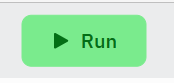
\includegraphics{Run}
    \caption{The Run button on Replit}
    \label{fig:Run}
\end{figure}

If you click that "Run" button, it will compile the code and run it. You should see the words "Hello World!" on the right side of the environment. Congratulations! You just created your first program!

As I mentioned, the C++ compiler is a real stickler for syntax.
If you make any errors when you type in the program, chances
are that it will not compile successfully.  For example, if
you misspell {\tt iostream}, you might get an error message like
the following:

\begin{verbatim}
hello.cpp:1: oistream.h: No such file or directory
\end{verbatim}
%
There is a lot of information on this line, but it is presented
in a dense format that is not easy to interpret.  A more friendly
compiler might say something like:

\begin{quote}
``On line 1 of the source code file named hello.cpp, you tried to
include a header file named oistream.h.  I didn't find anything
with that name, but I did find something named iostream.  Is
that what you meant, by any chance?''
\end{quote}

Unfortunately, few compilers are so accommodating.  The compiler
is not really very smart, and in most cases the error message
you get will be only a hint about what is wrong.  It will take
some time to gain facility at interpreting compiler messages.

Nevertheless, the compiler can be a useful tool for learning the
syntax rules of a language.  Starting with a working program
(like hello.cpp), modify it in various ways and see what happens.
If you get an error message, try to remember what the message says
and what caused it, so if you see it again in the future you
will know what it means.

\section{Exercises}
FIXME
Hello, I got this running (modified hello world)

\section{Glossary}

\begin{description}

\item[problem-solving:]  The process of formulating a problem, finding
a solution, and expressing the solution.

\item[high-level language:]  A programming language like C++ that
is designed to be easy for humans to read and write.

\item[low-level language:]  A programming language that is designed
to be easy for a computer to execute.  Also called ``machine
language'' or ``assembly language.''

\item[portability:]  A property of a program that can run on more
than one kind of computer.

\item[formal language:]  Any of the languages people have designed
for specific purposes, like representing mathematical ideas or
computer programs.  All programming languages are formal languages.

\item[natural language:]  Any of the languages people speak that
have evolved naturally.

\item[interpret:]  To execute a program in a high-level language
by translating it one line at a time.

\item[compile:]  To translate a program in a high-level language
into a low-level language, all at once, in preparation for later
execution.

\item[source code:]  A program in a high-level language, before
being compiled.

\item[object code:]  The output of the compiler, after translating
the program.

\item[executable:]  Another name for object code that is ready
to be executed.

\item[algorithm:]  A general process for solving a category of
problems. 

\item[bug:]  An error in a program.

\item[syntax:]  The structure of a program.

\item[semantics:]  The meaning of a program.

\item[parse:]  To examine a program and analyze the syntactic structure.

\item[syntax error:]  An error in a program that makes it impossible
to parse (and therefore impossible to compile).

\item[run-time error:]  An error in a program that makes it fail at
run-time.

\item[logical error:]  An error in a program that makes it do something
other than what the programmer intended.

\item[debugging:]  The process of finding and removing any of
the three kinds of errors.

\index{problem-solving}
\index{high-level language}
\index{low-level language}
\index{formal language}
\index{natural language}
\index{interpret}
\index{compile}
\index{syntax}
\index{semantics}
\index{parse}
\index{error}
\index{debugging}

\end{description}




% LaTeX source for textbook ``How to think like a computer scientist''
% Copyright (C) 2023  Lisa Patacchiola and Allen B Downey


\chapter{Variables and types}

\section{More output}
\index{output}
\index{statement!output}

As I mentioned in the last chapter, you can put as many statements as
you want in {\tt main}.  For example, to output more than one line:

\begin{mdframed}
\begin{verbatim}
#include <iostream>

// main: generate some simple output

int main ()
{
  std::cout << "Hello, world." << std::endl; // output 1 line
  std::cout << "How are you?" << std::endl;  // output 1 more
  return 0;
}
\end{verbatim}
%
\end{mdframed}

As you can see, it is legal to put comments at the
end of a line, as well as on a line by themselves.

If you want to try that with the replit code, go back to the link from the last chapter 
\url{https://replit.com/@lpatacch/helloWorld#hello.cpp}. Then, look for a button on the right hand of the screen with the words "Fork Repl". It should look like Figure \ref{fig:fork}
\begin{figure}
    \centering
    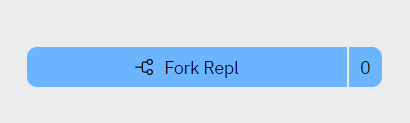
\includegraphics{fork}
    \caption{The Fork button on Replit}
    \label{fig:fork}
\end{figure}
You now should have a copy of the code that you can change any way you want.

\index{string}
\index{type!string}

In the program. the phrases that appear in quotation marks are called {\bf strings},
because they are made up of a sequence (string) of letters.  Actually,
strings can contain any combination of letters, numbers, punctuation
marks, and other special characters.

\index{newline}

Often it is useful to display the output from multiple output
statements all on one line.  You can do this by leaving out
the first {\tt endl}:

\begin{mdframed}

\begin{verbatim}
int main ()
{
  std::cout << "Goodbye, ";
  std::cout << "cruel world!" << std::endl;
  return 0
}
\end{verbatim}
%
\end{mdframed}
In this case the output appears on a single line as
{\tt Goodbye, cruel world!}.  Notice that there is a space
between the word ``Goodbye,'' and the second quotation mark.
This space appears in the output, so it affects the behavior
of the program.

Spaces that appear outside of quotation marks generally do
not affect the behavior of the program.  For example, I
could have written:

\begin{mdframed}

\begin{verbatim}
int main ()
{
  std::cout<<"Goodbye, ";
  std::cout<<"cruel world!"<<std::endl;
  return 0;
}
\end{verbatim}
%
\end{mdframed}
This program would compile and run just as well as the original.
The breaks at the ends of lines (newlines) do not affect
the program's behavior either, so I could have written:

\begin{mdframed}

\begin{verbatim}
int main(){std::cout<<"Goodbye, ";std::cout<<"cruel world!"
    <<std::endl;return 0;}
\end{verbatim}
%
\end{mdframed}
That would work, too, although you have probably noticed that
the program is getting harder and harder to read.  Newlines and
spaces are useful for organizing your program visually, making
it easier to read the program and locate syntax errors.

\section{Values}
\index{value}
\index{type}

A value is one of the fundamental things---like a letter or
a number---that a program manipulates.  The only values we have
manipulated so far are the string values we have been outputting, like
{\tt "Hello, world."}.  You (and the compiler) can identify
string values because they are enclosed in quotation marks.

There are other kinds of values, including integers and characters.
An integer is a whole number like 1 or 17.  You can output
integer values the same way you output strings:

\begin{mdframed}

\begin{verbatim}
  std::cout << 17 << std::endl;
\end{verbatim}
%

\end{mdframed}
A character value is a letter or digit or punctuation mark
enclosed in single quotes, like {\tt 'a'} or {\tt '5'}.
You can output character values the same way:


\begin{mdframed}

\begin{verbatim}
  std::cout << '}' << std::endl;
\end{verbatim}
%

\end{mdframed}
This example outputs a single close squiggly-brace on a line
by itself.

It is easy to confuse different types of values, like {\tt "5"}, {\tt
'5'} and {\tt 5}, but if you pay attention to the punctuation, it
should be clear that the first is a string, the second is a character
and the third is an integer.  The reason this distinction is important
should become clear soon.

\section {Variables}
\index{variable}
\index{value}

One of the most powerful features of a programming language is the
ability to manipulate {\bf variables}.  A variable is a named location
that stores a value.  

Just as there are different types of values (integer, character,
etc.), there are different types of variables.  When you create a new
variable, you have to declare what type it is.  For example, the
character type in C++ is called {\tt char}.  The following statement
creates a new variable named {\tt fred} that has type {\tt char}.

\begin{mdframed}

\begin{verbatim}
    char fred;
\end{verbatim}
%

\end{mdframed}
This kind of statement is called a {\bf declaration}.

The type of a variable determines what kind of values it can
store.  A {\tt char} variable can contain characters, and it should
come as no surprise that {\tt int} variables can store integers.

There are several types in C++ that can store string values, but we
are going to skip that for now (see Chapter~\ref{strings}).

\index{declaration}
\index{statement!declaration}

To create an integer variable, the syntax is 

\begin{mdframed}

\begin{verbatim}
  int bob;
\end{verbatim}
%

\end{mdframed}
where {\tt bob} is the arbitrary name you made up for the
variable.  In general, you will want to make up variable names
that indicate what you plan to do with the variable.  For
example, if you saw these variable declarations:

\begin{mdframed}

\begin{verbatim}
    char firstLetter;
    char lastLetter;
    int hour, minute;
\end{verbatim}
\end{mdframed}
%

you could probably make a good guess at what values
would be stored in them.  This example
also demonstrates the syntax for declaring multiple variables
with the same type: {\tt hour} and {\tt minute}
are both integers ({\tt int} type).

\section{Assignment}
\index{assignment}
\index{statement!assignment}

Now that we have created some variables, we would like to
store values in them.  We do that with an {\bf assignment
statement}.

\begin{mdframed}

\begin{verbatim}
    firstLetter = 'a';   // give firstLetter the value 'a'
    hour = 11;           // assign the value 11 to hour
    minute = 59;         // set minute to 59
\end{verbatim}
\end{mdframed}
%
This example shows three assignments, and the comments show
three different ways people sometimes talk about assignment
statements.  The vocabulary can be confusing here, but the
idea is straightforward:

\begin{itemize}

\item When you declare a variable, you create a named storage location.

\item When you make an assignment to a variable, you give it a value.

\end{itemize}

A common way to represent variables on paper is to draw a box
with the name of the variable on the outside and the value
of the variable on the inside.  This kind of figure is called
a {\bf state diagram} because is shows what state each of the
variables is in (you can think of it as the variable's ``state of
mind'').
This diagram shows
the effect of the three assignment statements:

\vspace{0.1in}
\centerline{\epsfig{figure=assign.eps}}
\vspace{0.1in}

\index{rules!variable value}
I sometimes use different shapes to indicate different
variable types.  These shapes should help remind you that one of the
rules in C++ is that a variable has to have the same type as the
value you assign it.  For example, you cannot store a string in
an {\tt int} variable.  The following statement generates a compiler
error.

\begin{mdframed}

\begin{verbatim}
  int hour;
  hour = "Hello.";       // WRONG !!
\end{verbatim}

\end{mdframed}
%
This rule is sometimes a source of confusion, because there are many
ways that you can convert values from one type to another, and C++
sometimes converts things automatically.  But for now you should
remember that as a general rule variables and values have the same
type, and we'll talk about special cases later.

Another source of confusion is that some strings {\em look}
like integers, but they are not.  For example,
the string {\tt "123"}, which is made up of the
characters {\tt 1}, {\tt 2} and {\tt 3}, is not
the same thing as the {\em number} {\tt 123}.
This assignment is illegal:

\begin{verbatim}
  minute = "59";         // WRONG!
\end{verbatim}
%
\section{Outputting variables}
\label{output}

You can output the value of a variable using the same commands
we used to output simple values.
\begin{mdframed}
\begin{verbatim}
  int hour, minute;
  char colon;

  hour = 11;
  minute = 59;
  colon = ':';

  std::cout << "The current time is ";
  std::cout << hour;
  std::cout << colon;
  std::cout << minute;
  std::cout << sts::endl;
\end{verbatim}
\end{mdframed}
%
Try this project here: \url{https://replit.com/@lpatacch/OutputVariables#main.cpp}.
This program creates two integer variables named {\tt hour} and {\tt
minute}, and a character variable named {\tt colon}.  It assigns
appropriate values to each of the variables and then uses a series
of output statements to generate the following:

\begin{verbatim}
The current time is 11:59
\end{verbatim}

When we talk about ``outputting a variable,'' we mean outputting the
{\em value} of the variable.  To output the {\em name} of a variable,
you have to put it in quotes.  For example: {\tt std::cout << "hour";}

As we have seen before, you can include more than one value in
a single output statement, which can make the previous program more
concise:

\begin{mdframed}

\begin{verbatim}
  int hour, minute;
  char colon;

  hour = 11;
  minute = 59;
  colon = ':';

  std::cout << "The current time is " << hour << colon 
                << minute << std::endl;
\end{verbatim}
\end{mdframed}
%
On one line, this program outputs a string, two integers, a character,
and the special value {\tt endl}.  Very impressive!


\section{Variable Naming Rules}
\index{variable naming rules}
\index{variable!naming rules}
\index{rules!variable naming}
A few sections ago, I said that you can make up any name you
want for your variables, but that's not quite true. There are certain rules that you need to follow.
\begin{enumerate}
    \item The name can not start with a number. (It is ok for a number to be in the name, it just can't be the first letter.)
    \item No spaces in the name
    \item Capitalization matters (num is different than NUM) 
    \item No special characters can be in the name other than underscore.
\end{enumerate}

Here are some examples of variables that do not follow the naming rules, and what you can use instead
\begin{mdframed}
\begin{verbatim}
    int 3player;    \\ WRONG, can not start with a number
    int player3;    \\ This would work
    int my3player   \\ This will also work
    
    int hit points; \\ WRONG, spaces not allowed in the name
    int hitPoints;  \\ This would work
    int hit_points; \\ This also would work
    
    int cash$;      \\ This would not work because of $sign
    int cashMoney;  \\ changed to use words instead
\end{verbatim}
\end{mdframed}
\subsection{Keywords}
\index{keyword}
In addition, there
are certain words that are reserved in C++ because they are
used by the compiler to parse the structure of your program,
and if you use them as variable names, it will get confused.
These words, called {\bf keywords}, include {\tt int},
{\tt char}, {\tt void}, {\tt endl} and many more.

The complete list of keywords is included in the C++ Standard, which
is the official language definition adopted by the the International
Organization for Standardization (ISO) on September 1, 1998.  You
can download a copy electronically from

    \url{http://www.ansi.org/}

%
Rather than memorize the list, I would suggest that you
take advantage of a feature provided in many development
environments: code highlighting.  As you type, different
parts of your program should appear in different colors.  For
example, keywords might be blue, strings red, and other code
black.  If you type a variable name and it turns blue, watch
out!  You might get some strange behavior from the compiler.

\section{Operators}
\index{operator}

{\bf Operators} are special symbols that are used to represent
simple computations like addition and multiplication.  Most
of the operators in C++ do exactly what you would expect them
to do, because they are common mathematical symbols.  For
example, the operator for adding two integers is {\tt +}.

The following are all legal C++ expressions whose meaning is
more or less obvious:

\begin{verbatim}
1+1        hour-1       hour*60 + minute     minute/60
\end{verbatim}
%
Expressions can contain both variables
names and integer values.  In each case the name of the variable is
replaced with its value before the computation is performed.

\index{expression}

\subsection{Not all the math operators}
Although some of the arithmetic operators that you would expect are there, there are some that do not work in C++. Here are a few examples of what does not work, and how to write it in a different way.

\begin{mdframed}
\begin{verbatim}
    int powerUpLevel = 2;
    int damageLevel = 3;
    
    int damageGiven = powerUpLeveldamageLevel;     // WRONG 
        // You can't just put variables next to each other
        // to have them multiply
        
    int damageGiven = powerUpLevel x damageLevel;  // WRONG 
        // You can't use x as a multiplication sign. It is
        // often used as a variable
        
    int damageGiven = powerUpLevel * damageLevel; // Correct!
        // When you multiply, you should use the * symbol
    
    int valToPower = powerUpLevel^2;              // WRONG
        // Although you can use the ^ symbol for a 
        // particular math operation, it is not to 
        // calculate the square (or any other power)
        // We will see this later in the book
        
    int valToPower = powerUpLevel * powerUpLevel; // Correct! 
        // To square a number, you can multiply it with
        // itself
        // There is also another way to do this which we
        // will see later
        
    int percentHurt = damageGiven ÷ 100;         // WRONG
        // C++ does not use this division sign
    
    int percentHurt = damageGiven/100;           // Correct
        // To divide, we should use the / symbol
        // There is something about this that is an issue,
        // that we will talk about right now.
\end{verbatim}
\end{mdframed}
%

\subsection{Integer Division}
Addition, subtraction and multiplication all do what you
expect, but you might be surprised by division.  For example,
the following program:

\begin{mdframed}

\begin{verbatim}
  int hour, minute;
  hour = 11;
  minute = 59;
  std::cout << "Number of minutes since midnight: ";
  std::cout << hour*60 + minute << std::endl;
  std::cout << "Fraction of the hour that has passed: ";
  std::cout << minute/60 << std::endl;
\end{verbatim}
\end{mdframed}
%

would generate the following output:

\begin{verbatim}
  Number of minutes since midnight: 719
  Fraction of the hour that has passed: 0
\end{verbatim}
%
Try it yourself here: \url{https://replit.com/@lpatacch/IntegerDivision#main.cpp}.
The first line is what we expected, but the second line is
odd.  The value of the variable {\tt minute} is 59, and
59 divided by 60 is 0.98333, not 0.  The reason for the
discrepancy is that C++ is performing {\bf integer division}.

\index{type!int}
\index{integer division}
\index{arithmetic!integer}
\index{division!integer}
\index{operand}

When both of the {\bf operands} are integers (operands are the things
operators operate on), the result must also be an integer,
and by definition integer division always rounds {\em down},
even in cases like this where the next integer is so close.

A possible alternative in this case is to calculate a percentage
rather than a fraction:

\begin{mdframed}
\begin{verbatim} 
  std::cout << "Percentage of the hour that has passed: ";
  std::cout << minute*100/60 << std::endl;
\end{verbatim}
\end{mdframed}

%
The result is:

\begin{verbatim}
    Percentage of the hour that has passed: 98
\end{verbatim}
%
Again the result is rounded down, but at least now the answer
is approximately correct.  In order to get an even more accurate
answer, we could use a different type of variable, called
floating-point, that is capable of storing fractional values.
We'll get to that in the next chapter.

\subsection{Modulus operator}
\label{modulus}
\index{modulus}
\index{remainder}
\index{operator!modulus}
\index{operator!remainder}
There is another way to get the information that the integer division is not using. That is a new operator called the {\bf modulus}, or {\bf remainder} operator.

The modulus operator works on integers (and integer expressions)
and yields the {\em remainder} when the first operand is divided
by the second.  In C++, the modulus operator is a percent sign,
{\tt \%}.  The syntax is exactly the same as for other operators:

\begin{verbatim}
  int quotient = 7 / 3;
  int remainder = 7 % 3;
\end{verbatim}
%
The first operator, integer division, yields 2.  The second
operator yields 1.  Thus, 7 divided by 3 is 2 with 1 left over.

The modulus operator turns out to be surprisingly useful.  For
example, you can check whether one number is divisible by
another: if {\tt x \% y} is zero, then {\tt x} is divisible
by {\tt y}.

Also, you can use the modulus operator to extract the rightmost
digit or digits from a number.  For example, {\tt x \% 10} yields
the rightmost digit of {\tt x} (in base 10).  Similarly
{\tt x \% 100} yields the last two digits.

\section{Order of operations}
\index{precedence}
\index{rules!precedence}
\index{order of operations}

When more than one operator appears in an expression the order
of evaluation depends on the rules of {\bf precedence}.  A
complete explanation of precedence can get complicated, but
just to get you started:

\begin{itemize}

\item Multiplication and division (and modulus) happen before
addition and subtraction.  So {\tt 2*3-1} yields 5, not 4, and {\tt
2/3-1} yields -1, not 1 (remember that in integer division {\tt 2/3}
is 0).

\item If the operators have the same precedence they are evaluated
from left to right.  So in the expression {\tt minute*100/60},
the multiplication happens first, yielding {\tt 5900/60}, which
in turn yields {\tt 98}.  If the operations had gone from right
to left, the result would be {\tt 59*1} which is {\tt 59}, which
is wrong.

\item Any time you want to override the rules of precedence (or
you are not sure what they are) you can use parentheses.  Expressions
in parentheses are evaluated first, so {\tt 2 * (3-1)} is 4.
You can also use parentheses to make an expression easier to
read, as in {\tt (minute * 100) / 60}, even though it doesn't
change the result.

\end{itemize}

\section{Operators for characters}
\index{character operator}
\index{operator!character}

Interestingly, the same mathematical operations that work on
integers also work on characters.  For example,

\begin{verbatim}
  char letter;
  letter = 'a' + 1;
  std::cout << letter << std::endl;
\end{verbatim}
%
outputs the letter {\tt b}.  Although it is syntactically legal
to multiply characters, it is almost never useful to do it.

Earlier I said that you can only assign integer values to
integer variables and character values to character variables,
but that is not completely true.  In some cases, C++ converts
automatically between types.  For example, the following is
legal.

\begin{verbatim}
  int number;
  number = 'a';
  std::cout << number << std::endl;
\end{verbatim}
%
The result is 97, which is the number that is used internally
by C++ to represent the letter {\tt 'a'}.  However, it is
generally a good idea to treat characters as characters, and
integers as integers, and only convert from one to the other
if there is a good reason.

Automatic type conversion is an example of a common problem in designing a
programming language, which is that there is a conflict between {\bf
formalism}, which is the requirement that formal languages should have
simple rules with few exceptions, and {\bf convenience}, which is the
requirement that programming languages be easy to use in practice.

More often than not, convenience wins, which is usually good for
expert programmers, who are spared from rigorous but unwieldy
formalism, but bad for beginning programmers, who are often baffled
by the complexity of the rules and the number of exceptions.  In this
book I have tried to simplify things by emphasizing the rules and
omitting many of the exceptions.


\section{Composition}
\index{composition}
\index{expression}

So far we have looked at the elements of a programming
language---variables, expressions, and statements---in
isolation, without talking about how to combine them.

One of the most useful features of programming languages
is their ability to take small building blocks and
{\bf compose} them.  For example, we know how to multiply
integers and we know how to output values; it turns out we can
do both at the same time:

\begin{verbatim}
    std::cout << 17 * 3;
\end{verbatim}
%
Actually, I shouldn't say ``at the same time,'' since in reality
the multiplication has to happen before the output, but
the point is that any expression, involving numbers, characters,
and variables, can be used inside an output statement.  We've
already seen one example:

\begin{verbatim}
  std::cout << hour*60 + minute << std::endl;
\end{verbatim}
%
You can also put arbitrary expressions on the right-hand
side of an assignment statement:

\begin{verbatim}
  int percentage;
  percentage = (minute * 100) / 60;
\end{verbatim}
%
This ability may not seem so impressive now, but we will see
other examples where composition makes it possible
to express complex computations neatly and concisely.

WARNING: There are limits on where you can use certain
expressions; most notably, the left-hand side of an assignment
statement has to be a {\em variable} name, not an expression.
That's because the left side indicates the storage location
where the result will go.  Expressions
do not represent storage locations, only values.  So the
following is illegal:  {\tt minute+1 = hour;}.

\section{Glossary}

\begin{description}

\item[variable:] A named storage location for values.  All
variables have a type, which determines which values it can
store.

\item[value:] A letter, or number, or other thing that can be
stored in a variable.  

\item[type:] A set of values.  The types
we have seen are integers ({\tt int} in C++) and characters ({\tt
char} in C++).

\item[keyword:]  A reserved word that is used by the compiler
to parse programs.  Examples we have seen include {\tt int},
{\tt void} and {\tt endl}.

\item[statement:] A line of code that represents a command or
action.  So far, the statements we have seen are declarations,
assignments, and output statements.

\item[declaration:] A statement that creates a new variable and
determines its type.

\item[assignment:] A statement that assigns a value to a variable.

\item[expression:] A combination of variables, operators and
values that represents a single result value.  Expressions also
have types, as determined by their operators and operands.

\item[operator:] A special symbol that represents a simple
computation like addition or multiplication.

\item[modulus:]  An operator that works on integers and yields
the remainder when one number is divided by another.  In C++
it is denoted with a percent sign ({\tt \%}).

\item[operand:] One of the values on which an operator operates. 

\item[precedence:] The order in which operations are evaluated.

\item[composition:] The ability to combine simple
expressions and statements into compound statements and expressions
in order to represent complex computations concisely.

\index{variable}
\index{value}
\index{type}
\index{keyword}
\index{statement}
\index{assignment}
\index{expression}
\index{operator}
\index{modulus}
\index{operand}
\index{composition}

\end{description}



% LaTeX source for textbook ``ThinkCPP , a game perspective''
% Copyright (C) 2023  Lisa Patacchiola, Allen B. Downey


\chapter{Conditionals}
\label{conditional}

\section{Floating-point}
\index{floating-point number}
\index{type!double}
\index{double (floating-point)}
\label{floating-point}

In the last chapter we had some problems dealing with numbers
that were not integers.  We worked around the problem by measuring
percentages instead of fractions, but a more general solution is
to use floating-point numbers, which can represent fractions
as well as integers.  In C++, there are two floating-point types,
called {\tt float} and {\tt double}.  In this book we will use
{\tt double}s exclusively.

You can create floating-point variables and assign values to them
using the same syntax we used for the other types.  For example:

\begin{lstlisting}
  double pi;
  pi = 3.14159;
\end{lstlisting}
%
It is also legal to declare a variable and assign a value to it at the
same time:

\begin{lstlisting}
  int x = 1;
  string empty = "";
  double pi = 3.14159;
\end{lstlisting}
%
In fact, this syntax is quite common.  A combined declaration
and assignment is sometimes called an {\bf initialization}.

\index{initialization}

Although floating-point numbers are useful, they are
often a source of confusion because there seems to be an
overlap between integers and floating-point numbers.  For
example, if you have the value {\tt 1}, is that an integer,
a floating-point number, or both?

Strictly speaking, C++ distinguishes the integer value {\tt 1}
from the floating-point value {\tt 1.0}, even though they
seem to be the same number.  They belong to
different types, and strictly speaking, you are not allowed
to make assignments between types.  For example, the following
is illegal

\begin{lstlisting}
    int x = 1.1;
\end{lstlisting}
%
because the variable on the left is an {\tt int}
and the value on the right is a {\tt double}.  But it is easy
to forget this rule, especially because there are places where C++
automatically converts from one type to another.
For example,

\begin{lstlisting}
    double y = 1;
\end{lstlisting}
%
should technically not be legal, but C++ allows it by converting the
{\tt int} to a {\tt double} automatically.  This leniency is
convenient, but it can cause problems; for example:

\begin{lstlisting}
    double y = 1 / 3;
\end{lstlisting}
%
You might expect the variable {\tt y} to be given the value
{\tt 0.333333}, which is a legal floating-point value, but in
fact it will get the value {\tt 0.0}.  The reason is that the
expression on the right appears to be the ratio of two integers,
so C++ does {\em integer} division, which yields the integer
value {\tt 0}.  Converted to floating-point, the result is
{\tt 0.0}.

One way to solve this problem (once you figure out what
it is) is to make the right-hand side a floating-point
expression:

\begin{lstlisting}
    double y = 1.0 / 3.0;
\end{lstlisting}
%
This sets {\tt y} to {\tt 0.333333}, as expected.

\index{arithmetic!floating-point}

All the operations we have seen---addition, subtraction,
multiplication, and division---work on floating-point values,
although you might be interested to know that the underlying mechanism
is completely different.  In fact, most processors have special
hardware just for performing floating-point operations.

\subsection{Converting from {\tt double} to {\tt int}}
\label{rounding}
\index{rounding}
\index{typecasting}
\index{static cast}
\index{cast!static}

As I mentioned, C++ converts {\tt int}s
to {\tt double}s automatically if necessary, because no
information is lost in the translation.  On the other hand,
going from a {\tt double} to an {\tt int} requires rounding
off.  C++ doesn't perform this operation automatically, in
order to make sure that you, as the programmer, are aware
of the loss of the fractional part of the number.

The simplest way to convert a floating-point value to an integer is to
use a {\bf typecast}.  Typecasting is so called because it allows you
to take a value that belongs to one type and ``cast'' it into another
type (in the sense of molding or reforming, not throwing).

The syntax for typecasting is different than code we have seen so far.  For example:

FIXME ADD more about STATIC CAST HERE
\begin{lstlisting}
  double pi = 3.14159;
  int x = static_cast<int>(pi);
\end{lstlisting}
%
The {\tt static\_cast<int>} function returns an integer, so {\tt x} gets the value
3.  Converting to an integer always rounds down, even if the fraction
part is 0.99999999.

For every type in C++, there is a corresponding function that
typecasts its argument to the appropriate type.

\section{Conditional execution}
\index{conditional}
\index{statement!conditional}

In order to write useful programs, we almost always need the ability
to check certain conditions and change the behavior of the program
accordingly.  {\bf Conditional statements} give us this ability.  The
simplest form is the {\tt if} statement:

\begin{lstlisting}
  if (x > 0) {
    std::cout << "x is positive" << std::endl;
  }
\end{lstlisting}
%
The expression in parentheses is called the condition.
If it is true, then the statements in brackets get executed.
If the condition is not true, nothing happens.

\index{operator!comparison}
\index{comparison!operator}

The condition can contain any of the {\tt comparison operators}:

\begin{lstlisting}
    x == y           // x equals y
    x != y           // x is not equal to y
    x > y            // x is greater than y
    x < y            // x is less than y
    x >= y           // x is greater than or equal to y
    x <= y           // x is less than or equal to y
\end{lstlisting}
%
Although these operations are probably familiar to you, the
syntax C++ uses is a little different from mathematical
symbols like $=$, $\neq$ and $\le$.  A common error is
to use a single {\tt =} instead of a double {\tt ==}.  Remember
that {\tt =} is the assignment operator, and {\tt ==} is
a comparison operator.  Also, there is no such thing as
{\tt =<} or {\tt =>}.

Unfortunately, the default behavior in many compilers is to not display warnings when you use one equal instead of two in an if statements. (Check out Chapter \ref{showwarning} if you want to know how to turn on the warnings.) Be sure to be careful when you are using equal signs and if statements.

The two sides of a condition operator have to be the same
type.  You can only compare {\tt ints} to {\tt ints} and
{\tt doubles} to {\tt doubles}. 

\section {Alternative execution}
\label{alternative}
\index{conditional!alternative}

A second form of conditional execution is alternative execution,
in which there are two possibilities, and the condition determines
which one gets executed.  The syntax looks like:

\begin{lstlisting}
    
  if (x%2 == 0) {
    std::cout << "x is even" << std::endl;
  } else {
    std::cout << "x is odd" << std::endl;
  }
\end{lstlisting}
%
(If you do not remember what the \% sign is doing, check out the
Modulus section in Chapter~\ref{modulus})
If the remainder when {\tt x} is divided by 2 is zero, then
we know that {\tt x} is even, and this code displays a message
to that effect.  If the condition is false, the second
set of statements is executed.  Since the condition must
be true or false, exactly one of the alternatives will be
executed.



\section {Chained conditionals}
\index{conditional!chained}

Sometimes you want to check for a number of related conditions
and choose one of several actions.  One way to do this is by
{\bf chaining} a series of {\tt if}s and {\tt else}s:

\begin{verbatim}
  if (x > 0) {
    cout << "x is positive" << endl;
  } else if (x < 0) {
    cout << "x is negative" << endl;
  } else {
    cout << "x is zero" << endl;
  }
\end{verbatim}
%
These chains can be as long as you want, although they can
be difficult to read if they get out of hand.  One way to
make them easier to read is to use standard indentation,
as demonstrated in these examples.  If you keep all the
statements and squiggly-braces lined up, you are less
likely to make syntax errors and you can find them more
quickly if you do.

\section{Nested conditionals}
\index{conditional!nested}

In addition to chaining, you can also nest one conditional
within another.  We could have written the previous example
as:

\begin{verbatim}
  if (x == 0) {
    cout << "x is zero" << endl;
  } else {
    if (x > 0) {
      cout << "x is positive" << endl;
    } else {
      cout << "x is negative" << endl;
    }
  }
\end{verbatim}
%
There is now an outer conditional that contains two branches.  The
first branch contains a simple output statement, but the second
branch contains another {\tt if} statement, which has two branches
of its own.  Fortunately, those two branches are both output
statements, although they could have been conditional statements as
well.

Notice again that indentation helps make the structure
apparent, but nevertheless, nested conditionals get difficult to read
very quickly.  In general, it is a good idea to avoid them when you
can.

\index{nested structure}

On the other hand, this kind of {\bf nested structure} is common, and
we will see it again, so you better get used to it.

\section{Logical operators}
\index{logical operator}
\index{operator!logical}
Nested if statements can get tricky to look at, so there are a couple of different ways to make it look less complex. The first we will look at is "logical operators".
There are three {\bf logical operators} in C++: AND, OR and NOT,
which are denoted by the symbols {\tt \&\&}, {\tt ||} and
{\tt !}.  The semantics (meaning) of these operators is similar
to their meaning in English.  For example {\tt x > 0 \&\& x < 10}
is true only if {\tt x} is greater than zero AND less than 10.

\index{semantics}

{\tt evenFlag || n\%3 == 0} is true if {\em either} of
the conditions is true, that is, if {\tt evenFlag} is true OR the
number is divisible by 3.

Finally, the NOT operator has the effect of negating or
inverting a bool expression, so {\tt !evenFlag} is true
if {\tt evenFlag} is false; that is, if the number is odd.

\index{nested structure}

Logical operators often provide a way to simplify nested
conditional statements.  For example, how would you write
the following code using a single conditional?

\begin{verbatim}
  if (x > 0) {
    if (x < 10) {
      cout << "x is a positive single digit." << endl;
    }
  }
\end{verbatim}

\section{{\tt switch} statement}
\index{switch statement}
\index{statement!switch}
\label{switch}

Another method that we can use instead of a complex if statement is {\tt switch}
statements.  A {\tt switch} statement
is an alternative to a chained conditional that is syntactically
prettier and often more efficient.  It looks like this:

\begin{verbatim}
  switch (symbol) {
  case '+':
    perform_addition ();
    break;
  case '*':
    perform_multiplication ();
    break;
  default:
    cout << "I only know how to perform addition and multiplication" << endl;
    break;
  }
\end{verbatim}
%
This {\tt switch} statement is equivalent to the following chained
conditional:

\begin{verbatim}
  if (symbol == '+') {
    perform_addition ();
  } else if (symbol == '*') {
    perform_multiplication ();
  } else {
    cout << "I only know how to perform addition and multiplication" << endl;
  }
\end{verbatim}
%
The {\tt break} statements are necessary in each branch
in a {\tt switch} statement because otherwise the flow of execution
``falls through'' to the next case.  Without the {\tt break} statements,
the symbol {\tt +} would make the program perform addition, and
then perform multiplication, and then print the error message.
Occasionally this feature is useful, but most of the time it is
a source of errors when people forget the {\tt break} statements.

\index{break statement}
\index{statement!break}

\index{default}

In general it is good style to include a {\tt default} case in
every {\tt switch} statement, to handle errors or unexpected values.

\section{Pseudocode}
\section{Flowcharts}
\section{Glossary}

\begin{description}
\item[floating-point:] A type of variable (or value) that can contain
fractions as well as integers.  There are a few floating-point types
in C++; the one we use in this book is {\tt double}.

\item[conditional:]  A block of statements that may or may not
be executed depending on some condition.

\item[chaining:]  A way of joining several conditional statements
in sequence.

\item[nesting:] Putting a conditional statement inside one or both
branches of another conditional statement.

\item[switch statement:] A different way to write conditional code. The switch selects the case to run depending on the variable it is checking.

\index{conditional}
\index{conditional!chained}
\index{conditional!nested}
\index{floating-point}
\index{switch statement}

\end{description}



% LaTeX source for textbook ``ThinkCPP , a game perspective''
% Copyright (C) 2023  Lisa Patacchiola and Allen B Downey

\chapter{Iteration}
\index{iteration}

One of the things computers are often used for is the automation
of repetitive tasks.  Repeating identical or similar tasks without
making errors is something that computers do well and people do
poorly.

The
type of repetition we will be looking at now is called {\bf iteration}, and C++ provides
several language features that make it easier to write iterative
programs.

The three features we are going to look at are the {\tt while}
statement, the {\tt do-while} statement, and the {\tt for} statement. There are another features, like the for-each and ranged based for loop, that we will cover in another chapter.

\section{The {\tt while} statement}
\index{statement!while}
\index{while statement}

Using a {\tt while} statement, we can write a countdown. What we would want to do is start with a certain number, then have the number go down (and print it out) while it is above zero. Then, print Blastoff!.

Here is pseudocode for that:
\begin{verbatim}
Set n to 3
WHILE n is more than zero
    print n
    subtract 1 from n
ENDWHILE
print "Blastoff!"
\end{verbatim}

Next, we can convert this to C++ code. It is not that much different than the pseudocode. Just like if statements, while statements use conditions to know when to continue and when to end. As long as the condition after the {\tt while} is true, the loop will continue to run. Once it is false, the loop will stop.

\begin{lstlisting}
  n = 3;
  while (n > 0) {
    std::cout << n << std::endl;
    n = n-1;
  }
  std::cout << "Blastoff!" << std::endl;
\end{lstlisting}
%
You can almost read a {\tt while} statement as if it were
English.  What this means is, ``While {\tt n} is greater than
zero, continue displaying the value of {\tt n} and then reducing
the value of {\tt n} by 1.  When you get to zero, output the
word `Blastoff!'''

This can be drawn as the following flowchart. 
\begin{figure}[h]
    \centering
    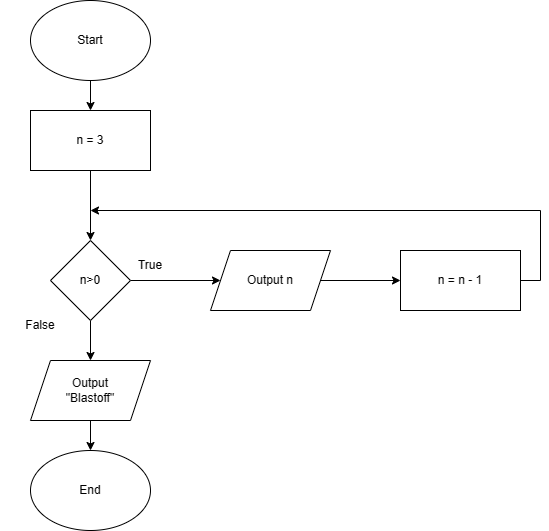
\includegraphics[width=9cm]{images/countdownwhileflow.png}
    \caption{Flowchart for the countdown program}
    \label{fig:countdownwhile}
\end{figure}
It is a little easier to understand how the code is looping by looking at the flowchart. Notice how after the n has one subtracted from it, the condition is checked again. That is the spot where it decides if the program will continue with the loop or end the loop.

More formally, the flow of execution for a {\tt while} statement
is as follows:

\begin{enumerate}

\item Evaluate the condition in parentheses, yielding {\tt true}
or {\tt false}.

\item If the condition is false, exit the {\tt while} statement
and continue execution at the next statement.

\item If the condition is true, execute each of the statements
between the curly-braces, and then go back to step 1.

\end{enumerate}

This type of flow is called a {\bf loop} because the third step loops
back around to the top.  Notice that if the condition is false the
first time through the loop, the statements inside the loop are
never executed.  The statements inside the loop are called
the {\bf body} of the loop.


\index{loop}
\index{loop!body}
\index{loop!infinite}
\index{body!loop}
\index{infinite loop}

The body of the loop should change the value of
one or more variables so that, eventually, the condition becomes
false and the loop terminates.  Otherwise the loop will repeat
forever, which is called an {\bf infinite loop}.  An endless
source of amusement for computer scientists is the observation
that the directions on shampoo, ``Lather, rinse, repeat,'' are
an infinite loop.

In the case of {\tt countdown}, we can prove that the loop
will terminate because we know that the value of {\tt n} is
finite, and we can see that the value of {\tt n} gets smaller
each time through the loop (each {\bf iteration}), so
eventually we have to get to zero.  In other cases it is not
so easy to tell:

\begin{verbatim}
    while (n != 1) {
      cout << n << endl;
      if (n%2 == 0) {           // n is even
        n = n / 2;
      } else {                  // n is odd
        n = n*3 + 1;
      }
    }

\end{verbatim}
%
The condition for this loop is {\tt n != 1}, so the loop
will continue until {\tt n} is 1, which will make the condition
false.

At each iteration, the program outputs the value of {\tt n} and then
checks whether it is even or odd.  If it is even, the value of
{\tt n} is divided by two.  If it is odd, the value is replaced
by $3n+1$.  For example, if the starting value (the argument passed
to {\tt sequence}) is 3, the resulting sequence is
3, 10, 5, 16, 8, 4, 2, 1.

Since {\tt n} sometimes increases and sometimes decreases, there is no
obvious proof that {\tt n} will ever reach 1, or that the program will
terminate.  For some particular values of {\tt n}, we can prove
termination.  For example, if the starting value is a power of two, then
the value of {\tt n} will be even every time through the loop, until
we get to 1.  The previous example ends with such a sequence,
starting with 16.

Particular values aside, the interesting question is whether
we can prove that this program terminates for {\em all} values of n.
So far, no one has been able to prove it {\em or} disprove it!

This book has a while loop simulator in order to help you understand while loops, \url{https://lpatacch.github.io/thinkCPPGamesEx/WhilePractice.html}. 
With this, you can change the 
initial value, the condition it is checking (\textless, \textgreater, ==, !=, \textgreater=, \textless=), the value checked,
and how the variable will change. Use this as many times as you wish
to understand how while loops work.
\section{New Operators}
Before we get more into loops, I want to cover some more math operators that we have not seen yet. In the countdown program, we had the counter change values with this equation:
\begin{verbatim}
    n = n-1;
\end{verbatim}
That equation took whatever was in n, subtracted 1, and placed it back in n. That behavior is very typical with loops. One variable 
is changed until it reaches the end value. It is so common that there is a short cut for this behavior. The above equation can be rewritten to this:
\begin{verbatim}
    n -= 1;
\end{verbatim}
This equation means the same as above, the value n has 1 subtracted from it, and then the result is put in n. Similar equations are available for many other math operators:
\begin{table}[h]
    \centering
    \begin{tabular}{|c|c|c|}
    \hline
 Math Operator & What it does & sample equation \\\hline
    +=     &  addition & {\tt n += 3;} \\
    -=      & subtraction & {\tt n -= 5;}\\
    {\tt *=}  &   multiplication & {\tt n *= 4;} \\
    \textbackslash=  &    division  & {\tt n \textbackslash= 2;}\\
    \%=  &  modulus & {\tt n \%= 7;}\\
\hline
    \end{tabular}
    \caption{New operators}
    \label{tab:newoperators}
\end{table}
\section{Increment and decrement operators}
\index{operator!increment}
\index{operator!decrement}

Incrementing and decrementing by one are such common operations that C++
provides special operators for them.  The {\tt ++} operator adds one
to the current value of an {\tt int}, {\tt char} or {\tt double}, and
{\tt --} subtracts one.  Neither operator works on {\tt string}s,
and neither {\em should} be used on {\tt bool}s.

The equation we modified in the last section:
\begin{verbatim}
    n -= 1;
\end{verbatim}

If you notice, the n was decremented by one. So, we can use the even shorter form here:
\begin{verbatim}
    --n;
\end{verbatim}
This subtracts 1 from n. This makes a very small line of code. All you need is the increment or the decrement operator, and the variable you will be changing.

You may have noticed that on some lines I put the ++ before the variable, and some after the variable. Both are legal. When it is on it's own line, it seems like it is doing the same thing. But, it is doing something slightly different. The ++ before the variable is called a pre-incrementor. It means that it will be doing the adding before anything else in the line. The ++ after the variable is called a post-incrementor. It means that it will be doing the adding after most of the things on the line. 

Technically, it is legal to increment a variable and use it
in an expression at the same time.  For example, you might see
something like:

\begin{verbatim}
  std::cout << i++ << std::endl;
\end{verbatim}
%
Looking at this, it is not clear whether the increment will
take effect before or after the value is displayed.  Because
expressions like this tend to be confusing, I would discourage
you from using them.  In fact, to discourage you even more,
I'm not going to tell you what the result is, other than letting you know it is a post-incrementor.  If you really
want to know, you can try it.

Using the increment operators, we can calculate the average weight of a person's inventory:

\begin{lstlisting}
  
  int num = 0;
  int weight = 0;
  int total = 0;
  std::cout << "Enter the weight of the item.\n"
  std::cout << "When done, enter -1\n";
  std::cin >> weight;
  while (weight >= 0) {
    //if it is a valid weight, add it to the total
    total += weight;
    
    //add one to the number of items
    ++num;
    
    //ask for the next weight
    std::cout << "Enter the weight of the item.\n"
    std::cout << "When done, enter -1\n";
    std::cin >> weight;    
  }
  
  if (num != 0)
  {
    std::cout << "The average is" << total/num <<".\n"; 
  }
  else {
    std::cout << "No items to average.\n";
  }
\end{lstlisting}
%
It is a common error to write something like

\begin{verbatim}
  num = num++;             // WRONG!!
\end{verbatim}
%
Unfortunately, this is syntactically legal, so the compiler
will not warn you.  The effect of this statement is to leave
the value of {\tt num} unchanged.  This is often a difficult
bug to track down.

Remember, you can write {\tt num = num +1;}, or you
can write {\tt num++;}, but you shouldn't mix them.

The ++ and -- does not work on a complex expression either. For example, 

\begin {verbatim}
( n + 7 )++;
\end{verbatim}
would not compile. The ++ and -- should be used only on a variable, not an expression.

\section{Parts of a loop}
The loops we have written so far have a number of elements
in common.  All of them start by initializing a variable;
they have a test, or condition, that depends on that variable;
and inside the loop they do something to that variable,
like increment it. This can be described by the following pseudocode:
\begin{verbatim}
  INITIALIZER;
  while (CONDITION) {
    BODY
    MODIFICATION
  }
\end{verbatim}
Loops, in order to work properly, need to have all three parts. If there is no modification section, the loop would never be able to leave the loop. If the initialization is wrong (or missing), the loop may loop the wrong amount of times (or never loop). And last, if the condition is wrong, the loop will never end properly. Whenever you loop is not working properly, if you look at those three parts, you will find the problem.

\section{Definite loop}
There are two different ways that loops can usually be identified. The first type 
is one where you know how many times the loop will repeat. These type of loops tend to
have a counter that is either counting down or up, and the counter is modified by a
constant value each time through the loop. These loops are sometimes called definite loops,
or counting loops. We have seen example with the countdown loop. The count down started at
three and the counter went down by one each time through the loop. Here is another example:

\begin{lstlisting}
  int val = 7;
  std::cout << "Here is a multiplication table for ";
  std::cout << val <<"\n";
  
  int x = 1;
  while (x <= 10)
  {
     std::cout << x << "\t" << x * val << "\n";
     x++;
  }
\end{lstlisting}
This loop has the condition as x<=10. If you look in the loop, you will notice that
x is being modified by 1 each time through the loop. Also, x is initialized to 1
when the loop starts. That means that the loop will repeat 10 times. Every time you
run this code, it will repeat 10 times.

In case you are interested, the \textbackslash t is one of the escape sequences that
we mentioned in \ref{tab:escapechar}. This spaces out each column by a tab stop. There 
are better ways to format tables, but we will not cover those methods for a while.

\section{Indefinite loop}
There is a different type of loop where you will not know how many times the loop
will run. The loop is checking a condition that will change, but it is different every
time we run the loop. We showed an example in the weight of the inventory code. This 
loop may have not repeated at all, or it could have repeated a thousand times. Since
you can not tell how many times it will repeat, it can be called an "indefinite loop". 
The number of repeats depended on what the user was entering. That code was waiting on a particular value (a negative number).
When a loop is waiting for a particular value, that value is called a flag, or a sentinel, which is why this loop may be
called a sentinel loop. 

FIXME: add an example

FIXME: code blocks
\section{{\tt do-while} loop}
The second type of loop that C++ supports is called a do-while loop.
It works very similarly to the while loop. It should be initialized
before the loop starts, it should be modified inside the loop, and
it has a condition it checks. The difference is where it checks the
condition. The do-while loop checks the condition at the end of the
loop, guaranteeing the loop always runs at least once. The while loop
checks the condition at the beginning, which could mean the loop
might not run at all. The general syntax looks like the following:

\begin{verbatim}
  INITIALIZER;
   do {
    BODY
    MODIFICATION
  } while (CONDITION);
\end{verbatim}
%

For example, the multiplication table could be changed to a do-while:
\begin{lstlisting}
  int val = 7;
  std::cout << "Here is a multiplication table for ";
  std::cout << val <<"\n";
  
  int x = 1;
  do {
     std::cout << x << "\t" << x * val << "\n";
     x++;
  } while (x <= 10);
\end{lstlisting}
\begin{figure}[h]
    \centering
    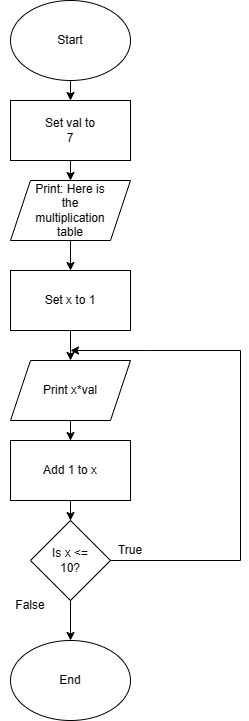
\includegraphics[height=10cm]{images/do-whileflow.png}
    \caption{Flowchart for the do-while multiplication table}
    \label{fig:do-while}
\end{figure}
By now, you may be wondering, "Why should I use this approach instead of a while loop?" The main advantage is that the code within the loop is guaranteed to execute at least once. I often use this type of loop when obtaining input from the user. In many programs, we ask a question. Unfortunately, the user may not always provide a valid response. While we know that we need to ask the question once, we cannot be certain if we will need to repeat it if the user provides an incorrect response. For instance, let's consider an example where we ask the user whether they want to turn left or right. The only correct answer is 'l' or 'r'. \footnote{Technically, we should have changed the answer to lowercase to allow for L and R,
but I wanted this example to be simpler than that.}
\begin{lstlisting}
  char direction = '\0';
  do {
     std::cout << "Do you want to go (l)eft or (r)ight?\n");
     std::cin >> direction;
     if ((direction != 'l')&&(direction != 'r'))
     {
        std::cout << "Please enter l or r\n";
     }
  } while ((direction != 'l')&&(direction != 'r'));
\end{lstlisting}
If we decided to do this with a while, we would have needed to ask 
the question both outside and inside the loop. This reduces the 
amount of times the same code is written in the program.

\section{{\tt for} loops}
\index{loop!for}
\index{for}
\index{statement!for}
We have had many examples of definite or counting loops.
This type of loop is so common that there is an alternate
loop statement, called {\tt for}, that expresses it more
concisely.  The general syntax looks like this:

\begin{verbatim}
  for (INITIALIZER; CONDITION; INCREMENTOR) {
    BODY
  }
\end{verbatim}
%
This statement is exactly equivalent to

\begin{verbatim}
  INITIALIZER;
  while (CONDITION) {
    BODY
    INCREMENTOR
  }
\end{verbatim}
%
except that it is more concise and, since it puts all the
loop-related statements in one place, it is easier to read.
For example:

\begin{verbatim}
  int i;
  for (i = 0; i < 4; i++) {
    cout << i << endl;
  }
\end{verbatim}
%
is equivalent to 

\begin{verbatim}
  int i = 0;
  while (i < 4) {
    cout << i << endl;
    i++;
  }
\end{verbatim}

FIXME - example of for loop with a decrement instead
FIXME - example of for loop with a step of 5

\section{Break and Continue}
FIXME add examples of how this works
\section{Glossary}

\begin{description}

\item[loop:]  A statement that executes repeatedly while a
condition is true or until some condition is satisfied.

\item[infinite loop:]  A loop whose condition is always true.

\item[body:]  The statements inside the loop.

\item[iteration:]  One pass through (execution of) the body
of the loop, including the evaluation of the condition.


\index{loop}
\index{infinite loop}
\index{body}
\index{loop!infinite}
\index{iteration}


\end{description}


% LaTeX source for textbook ``ThinkCPP , a game perspective''
% Copyright (C) 2023  Lisa Patacchiola 

\chapter{Game Loops}
FIXME - put the game loop information here
% LaTeX source for textbook ``ThinkCPP , a game perspective''
% Copyright (C) 2023 Lisa Patacchiola, Allen B. Downey

\chapter{Function}

\section{Math functions}
\index{math function}
\index{function!Math}
\index{expression}
\index{argument}
\label{mathlibrary}

In mathematics, you have probably seen functions like $\sin$ and
$\log$, and you have learned to evaluate expressions like
$\sin(\pi/2)$ and $\log(1/x)$.  First, you evaluate the
expression in parentheses, which is called the {\bf argument} of the
function.  For example, $\pi/2$ is approximately 1.571, and $1/x$ is
0.1 (if $x$ happens to be 10).

Then you can evaluate the function itself, either by looking it up in
a table or by performing various computations.  The $\sin$ of 1.571 is
1, and the $\log$ of 0.1 is -1 (assuming that $\log$ indicates the
logarithm base 10).

This process can be applied repeatedly to evaluate more complicated
expressions like $\log(1/\sin(\pi/2))$.  First we evaluate the
argument of the innermost function, then evaluate the function,
and so on.

C++ provides a set of built-in functions that includes most
of the mathematical operations you can think of.
The math functions are invoked using a syntax that is similar to
mathematical notation:

\begin{verbatim}
     double log = std::log (17.0);
     double angle = 1.5;
     double height = std::sin (angle);
\end{verbatim}
%
The first example sets {\tt log} to the logarithm of 17, base
$e$.  There is also a function called {\tt log10} that takes
logarithms base 10.

The second example finds the sine of the value of the variable
{\tt angle}.  C++ assumes that the
values you use with {\tt sin} and the other trigonometric functions
({\tt cos}, {\tt tan}) are in {\em radians}.  To
convert from degrees to radians, you can divide by 360
and multiply by $2 \pi$.  

If you don't happen to know $\pi$ to 15 digits, you can
calculate it using the {\tt acos} function.  The arccosine
(or inverse cosine) of -1 is $\pi$, because the cosine of
$\pi$ is -1.

\begin{verbatim}
  double pi = std::acos(-1.0);
  double degrees = 90;
  double angle = degrees * 2 * pi / 360.0;
\end{verbatim}
%
Before you can use any of the math functions, you have to
include the cmath {\bf header file}.  Header files contain
information the compiler needs about functions that are defined
outside your program.  For example, in the ``Hello, world!''
program we included a header file named {\tt iostream} using
an {\bf include} statement:

\begin{verbatim}
#include <iostream>
using namespace std;
\end{verbatim}
%
{\tt iostream} contains information about input and output
(I/O) streams, including the object named {\tt cout}.
C++ has a powerful feature called namespaces, that
allow you to write your own implementation of {\tt cout}.
But in most cases, we would need to use the standard implementation.
To convey this to the compiler, we use the line

\begin{verbatim}
using namespace std;
\end{verbatim}

To save yourself some typing, you can write {\tt using namespace std;} whenever
you use {\tt iostream}. This allows a shorthand where you can skip
typing the std:: in your code. For example, the hello world program
could be shortened to the following:
\begin{lstlisting}
#include <iostream>
using namespace std;

// main: generate some simple output
int main ()
{
  cout << "Hello, world." << endl;
  return 0;
}
\end{lstlisting}
%
However, in general it is not good practice, since it imports the 
entirety of std into your program.  This can become a problem when your programs get 
more complicated, and it takes over some of the namespace you would
want to use.
For this course it is an acceptable time-saving device, but I would
suggest you remove it for any portfolio projects. 

\index{header file}
\index{cmath}
\index{iostream}

Just like iostream, the math header file contains information
about the math functions.  You can include it at the beginning
of your program along with {\tt iostream}:

\begin{verbatim}
#include <cmath>
\end{verbatim}

Such header files have an initial `c' to signify that these
header files have been derived from the {\bf C} language.
\section{Math constants}
Although you can calculate PI using acos, C++ has done the calculation
ahead of time for you. If you are using C++20 or later, you can use the values in std::numbers. 

\begin{verbatim}
double mypi = std::numbers::pi;
\end{verbatim}
There are many other values available too, like e and phi.

If you are using an older version of the compilers, you may need to 
use a different technique to get PI. If you are including <cmath>, you should also have M\_PI defined.

\begin{verbatim}
double mypi = M_PI;
\end{verbatim}

If you have a very old version of C++, it may need a special line above the include cmath in order for M\_PI to work. But, I suggest you try the above versions
first before using this:

\begin{verbatim}
#define _USE_MATH_DEFINES
#include <cmath>
\end{verbatim}

\section {Composition}
\label{composition}
\index{composition}
\index{expression}

Just as with mathematical functions, C++ functions can be {\bf
composed}, meaning that you use one expression as part of another.
For example, you can use any expression as an argument to a function:

\begin{verbatim}
    double x = cos (angle + pi/2);
\end{verbatim}
%
This statement takes the value of {\tt pi}, divides it by two and
adds the result to the value of {\tt angle}.  The sum is
then passed as an argument to the {\tt cos} function.

You can also take the result of one function and pass it as
an argument to another:

\begin{verbatim}
    double x = exp (log (10.0));
\end{verbatim}
%
This
statement finds the log base $e$ of 10 and then raises $e$ to that
power.  The result gets assigned to {\tt x}; I hope you know what it
is.

\section{Adding new functions}
\index{function!definition}
\index{main}
\index{function!main}

So far we have only been using the functions that are built into C++,
but it is also possible to add new functions.  Actually, we have already
seen one function definition: {\tt main}.  The function named {\tt main}
is special because it indicates where the execution of the program
begins, but the syntax for {\tt main} is the same as for any other
function definition:

\begin{verbatim}
  void NAME ( LIST OF PARAMETERS ) {
    STATEMENTS
  }
\end{verbatim}
%
You can make up any name you want for your function, except
that you can't call it {\tt main} or any other
C++ keyword.  The list of
parameters specifies what information, if any, you have to
provide in order to use (or {\bf call}) the new function.

{\tt main} doesn't take any parameters, as indicated by
the empty parentheses {\tt ()} in it's definition\footnote{You can add parameters in main to get access to the command line parameters. We will show how to use them much later in the book. For now, it is OK to use main without parameters. }.  The first couple
of functions we are going to write also have no parameters, so the
syntax looks like this:

\begin{verbatim}
  void newLine () {
    std::cout << std::endl;
  }
\end{verbatim}
%
This function is named {\tt newLine}; it contains only a single
statement, which outputs a newline character, represented by
the special value {\tt endl}.

In {\tt main} we can call this new function using syntax that
is similar to the way we call the built-in C++ commands:

\begin{verbatim}
int main ()
{
  std::cout << "First Line." << std::endl;
  newLine ();
  std::cout << "Second Line." << std::endl;
  return 0;
}
\end{verbatim}
%
The output of this program is

\begin{verbatim}
First line.

Second line.
\end{verbatim}
%
Notice the extra space between the two lines.  What if we wanted
more space between the lines?  We could call the same
function repeatedly:

\begin{verbatim}
int main ()
{
  std::cout << "First Line." << std::endl;
  newLine ();
  newLine ();
  newLine ();
  std::cout << "Second Line." << std::endl;
  return 0;
}
\end{verbatim}
%

We could use a for loop to call it multiple times:
\begin{verbatim}
int main ()
{
  std::cout << "First Line." << std::endl;
  for (int x = 0; x < 3; x++) {
     newLine ();
  }
  std::cout << "Second Line." << std::endl;
  return 0;
}
\end{verbatim}
It is acceptable to have a function inside a loop. 
Or we could write a new function, named {\tt threeLine}, that 
prints three new lines:

\begin{verbatim}
void threeLine ()
{
  newLine ();  newLine ();  newLine ();
}

int main ()
{
  std::cout << "First Line." << std::endl;
  threeLine ();
  std::cout << "Second Line." << std::endl;
  return 0;
}
\end{verbatim}
%
You should notice a few things about this program:

\begin{itemize}

\item You can call the same procedure repeatedly.  In
fact, it is quite common and useful to do so.

\item You can have one function call another function.  In this
case, {\tt main} calls {\tt threeLine} and {\tt threeLine}
calls {\tt newLine}.  Again, this is common and useful.

\item In {\tt threeLine} I wrote three statements all on the
same line, which is syntactically legal (remember that spaces
and new lines usually don't change the meaning of a program).
On the other hand, it is usually a better idea to put each
statement on a line by itself, to make your program easy to
read.  I sometimes break that rule in this book to save space.

\end{itemize}

So far, it may not be clear why it is worth the trouble to
create all these new functions.  Actually, there are a lot
of reasons, but this example only demonstrates two:

\begin{enumerate}

\item Creating a new function gives you an opportunity to
give a name to a group of statements.  Functions can simplify a program
by hiding a complex computation behind a single command, and by using
English words in place of arcane code.  Which is clearer, {\tt
newLine} or {\tt cout << endl}?

\item Creating a new function can make a program smaller by eliminating
repetitive code.  For example, a short way to print nine consecutive
new lines is to call {\tt threeLine} three times.  How would you
print 27 new lines?

\end{enumerate}

\section {Definitions and uses}

Pulling together all the code fragments from the previous
section, the whole program looks like this:

\begin{verbatim}
#include <iostream>
using namespace std;

void newLine ()
{
  cout << endl;
}

void threeLine ()
{
  newLine ();  newLine ();  newLine ();
}

int main ()
{
  cout << "First Line." << endl;
  threeLine ();
  cout << "Second Line." << endl;
  return 0;
}
\end{verbatim}

This program contains three function definitions: {\tt newLine},
{\tt threeLine}, and {\tt main}.

Inside the definition of {\tt main}, there is a statement that
uses or calls {\tt threeLine}.  Similarly, {\tt threeLine} calls
{\tt newLine} three times.  Notice that the definition of each
function appears above the place where it is used.

This is necessary in C++; the definition of a function must
appear before (above) the first use of the function.  You
should try compiling this program with the functions in a
different order and see what error messages you get.

\section {Programs with multiple functions}

When you look at a class definition that contains several functions, it
is tempting to read it from top to bottom, but that is likely to be
confusing, because that is not the {\bf order of execution} of the
program.

Execution always begins at the first statement of {\tt main},
regardless of where it is in the program (often it is at the bottom).
Statements are executed one at a time, in order, until you reach a
function call.  Function calls are like a detour in the flow of
execution.  Instead of going to the next statement, you go to the
first line of the called function, execute all the statements there,
and then come back and pick up again where you left off.

That sounds simple enough, except that you have to remember that one
function can call another.  Thus, while we are in the middle of {\tt
main}, we might have to go off and execute the statements in {\tt
threeLine}.  But while we are executing {\tt threeLine}, we get
interrupted three times to go off and execute {\tt newLine}.

Fortunately, C++ is adept at keeping track of where it is, so
each time {\tt newLine} completes, the program picks up where it left
off in {\tt threeLine}, and eventually gets back to {\tt main} so the
program can terminate.

What's the moral of this sordid tale?  When you read a program, don't
read from top to bottom.  Instead, follow the flow of execution.

\section {Parameters and arguments}
\index{parameter}
\index{argument}

Some of the built-in functions we have used have {\bf parameters},
which are values that you provide to let the function do its
job.  For example, if you want to find the sine of a number,
you have to indicate what the number is.  Thus, {\tt sin}
takes a {\tt double} value as a parameter.

Some functions take more than one parameter, like {\tt pow},
which takes two {\tt doubles}, the base and the exponent.

Notice that in each of these cases we have to specify not
only how many parameters there are, but also what type they
are.  So it shouldn't surprise you that when you write a
class definition, the parameter list indicates the type of
each parameter.  For example:

\begin{verbatim}
  void printTwice (char phil) {
    cout << phil << phil << endl;
  }
\end{verbatim}
%
This function takes a single parameter, named {\tt phil}, that
has type {\tt char}.  Whatever that parameter is (and at
this point we have no idea what it is), it gets printed
twice, followed by a newline.
I chose the name {\tt phil} to suggest that the name
you give a parameter is up to you, but in general you want to
choose something more illustrative than {\tt phil}.

In order to call this function, we have to provide a {\tt char}.
For example, we might have a {\tt main} function like this:

\begin{verbatim}
  int main () {
    printTwice ('a');
    return 0;
  }
\end{verbatim}
%
The {\tt char} value you provide is called an {\bf argument}, and we
say that the argument is {\bf passed} to the function.  In this
case the value {\tt 'a'} is passed as an argument
to {\tt printTwice} where it will get printed twice.

Alternatively, if we had a {\tt char} variable, we could
use it as an argument instead:

\begin{verbatim}
  int main () {
    char argument = 'b';
    printTwice (argument);
    return 0;
  }
\end{verbatim}
%
Notice something very important here: the name of the variable we pass
as an argument ({\tt argument}) has nothing to do with the name of the
parameter ({\tt phil}).  Let me say that again:

\begin{quote}

{\bf The name of the variable we pass as an argument has nothing to do
with the name of the parameter.}

\end{quote}

They can be the same or they can be different, but it is important
to realize that they are not the same thing, except that they happen
to have the same value (in this case the character {\tt 'b'}).

The value you provide as an argument must have the same type as
the parameter of the function you call.  This rule is
important, but it is sometimes confusing because C++ sometimes
converts arguments from one type to another automatically.  For
now you should learn the general rule, and we will deal with
exceptions later.

\section {Parameters and variables are local}

Parameters and
variables only exist inside their own functions.  Within the
confines of {\tt main}, there is no such thing as {\tt phil}.
If you try to use it, the compiler will complain.  Similarly,
inside {\tt printTwice} there is no such thing as {\tt argument}.

Variables like this are said to be {\bf local}.  In order to
keep track of parameters and local variables, it is useful to
draw a {\bf stack diagram}.  Like state diagrams, stack diagrams
show the value of each variable, but the variables are contained
in larger boxes that indicate which function they belong to.

For example, the stack diagram for {\tt printTwice} looks like this in figure \ref{fig:stack}:

\vspace{0.1in}
\begin{figure}[h]
    \centering
    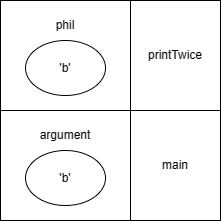
\includegraphics[height=6cm]{images/stack.png}
    \caption{Stack diagram from when printTwice is called}
    \label{fig:stack}
\end{figure}
%
Whenever a function is called, it creates a new {\bf instance}
of that function.  Each instance of a function contains the
parameters and local variables for that function.  In the
diagram an instance of a function is represented by a box
with the name of the function on the outside and the variables
and parameters inside.

In the example, {\tt main} has one local variable, {\tt argument}, and
no parameters.  {\tt printTwice} has no local variables and one
parameter, named {\tt phil}.

\section {Functions with multiple parameters}
\index{parameter!multiple}
\index{function!multiple parameter}
\index{class!Time}

The syntax for declaring and invoking functions with multiple
parameters is a common source of errors.  First, remember
that you have to declare the type of every parameter.  For
example

\begin{verbatim}
  void printTime (int hour, int minute) {
    cout << hour;
    cout << ":";
    cout << minute;
  }
\end{verbatim}
%
It might be tempting to write {\tt (int hour, minute)}, but
that format is only legal for variable declarations, not
for parameters.

Another common source of confusion is that you do not have
to declare the types of arguments.  The following is wrong!

\begin{verbatim}
    int hour = 11;
    int minute = 59;
    printTime (int hour, int minute);   // WRONG!
\end{verbatim}
%
In this case, the compiler can tell the type of {\tt hour}
and {\tt minute} by looking at their declarations.  It is
unnecessary and illegal to include the type when you pass them
as arguments.  The correct
syntax is {\tt printTime (hour, minute)}.

\label{printparity}
Do you remember the if/else code we did in the Chapter \ref{alternative} to check if something was even or odd? If you think you might want to check the parity
(evenness or oddness) of numbers often, you might want to
``wrap'' this code up in a function, as follows:

\begin{lstlisting}

void printParity (int x) {
  if (x%2 == 0) {
    std::cout << "x is even" << std::endl;
  } else {
    std::cout << "x is odd" << std::endl;
  }
}
\end{lstlisting}
%
Now you have a function named {\tt printParity} that will display
an appropriate message for any integer you care to provide. It is perfectly acceptable to have an if statement in a function.
In {\tt main} you would call this function as follows:

\begin{verbatim}
    printParity (17);
\end{verbatim}
%
Always remember that when you {\em call} a function, you do
not have to declare the types of the arguments you provide.
C++ can figure out what type they are.  You should resist the
temptation to write things like:

\begin{verbatim}
  int number = 17;
  printParity (int number);         // WRONG!!!
\end{verbatim}
\section {Functions with results}
\index{fruitful function}
\index{function!fruitful}

You might have noticed by now that some of the functions we are using,
like the math functions, yield results.  Other functions,
like {\tt newLine}, perform an action but
don't return a value.  That raises some questions:

\begin{itemize}

\item What happens if you call a function and you don't
do anything with the result (i.e. you don't assign it to
a variable or use it as part of a larger expression)?

\item What happens if you use a function without a result as part
of an expression, like {\tt newLine() + 7}?

\item Can we write functions that yield results, or are we
stuck with things like {\tt newLine} and {\tt printTwice}?

\end{itemize}

The answer to the third question is ``yes, you can write functions that
return values,'' and we'll do it in Chapter~\ref{fruitful functions}.  I will
leave it up to you to answer the other two questions by trying them
out.  Any time you have a question about what is legal or
illegal in C++, a good way to find out is to ask the compiler.

\section{The {\tt return} statement}
\index{return}
\index{statement!return}

The {\tt return} statement allows you to terminate the execution
of a function before you reach the end.  One reason to use it
is if you detect an error condition:

\begin{verbatim}
#include <cmath>

void printLogarithm (double x) {
  if (x <= 0.0) {
    cout << "Positive numbers only, please." << endl;
    return;
  }

  double result = log (x);
  cout << "The log of x is " << result;
}
\end{verbatim}
%
This defines a function named {\tt printLogarithm} that takes
a {\tt double} named {\tt x} as a parameter.  The first thing
it does is check whether {\tt x} is less than or equal to
zero, in which case it displays an error message and then uses
{\tt return} to exit the function.  The flow of execution
immediately returns to the caller and the remaining lines of
the function are not executed.

I used a floating-point value on the right side of the condition
because there is a floating-point variable on the left.

Remember that any time you want to use one a function from the math
library, you have to include the header file {\tt cmath}.

\section{Recursion}
\label{recursion}
\index{recursion}

I mentioned in the last chapter that it is legal for one function to
call another, and we have seen several examples of that.  I neglected
to mention that it is also legal for a function to call itself.  It
may not be obvious why that is a good thing, but it turns out to be
one of the most magical and interesting things a program can do.

For example, look at the following function:

\begin{verbatim}
void countdown (int n) {
  if (n == 0) {
    cout << "Blastoff!" << endl;
  } else {
    cout << n << endl;
    countdown (n-1);
  }
}
\end{verbatim}
%
The name of the function is {\tt countdown} and it takes a single
integer as a parameter.  If the parameter is zero, it outputs
the word ``Blastoff.''  Otherwise, it outputs the parameter and
then calls a function named {\tt countdown}---itself---passing
{\tt n-1} as an argument.

What happens if we call this function like this:

\begin{verbatim}
#include <iostream>
#include <cmath>
using namespace std;
void printLogarithm (double x) {
  if (x <= 0.0) {
    cout << "Positive numbers only, please." << endl;
    return;
  }

  double result = log (x);
  cout << "The log of x is " << result;
}

void countdown (int n) {
  if (n == 0) {
    cout << "Blastoff!" << endl;
  } else {
    cout << n << endl;
    countdown (n-1);
  }
}

int main ()
{
  countdown (3);
  return 0;
}
\end{verbatim}
%
The execution of {\tt countdown} begins with {\tt n=3}, and
since {\tt n} is not zero, it outputs the value 3, and then
calls itself...

\begin{quote}
The execution of {\tt countdown} begins with {\tt n=2}, and
since {\tt n} is not zero, it outputs the value 2, and then
calls itself...

\begin{quote}
The execution of {\tt countdown} begins with {\tt n=1}, and
since {\tt n} is not zero, it outputs the value 1, and then
calls itself...

\begin{quote}
The execution of {\tt countdown} begins with {\tt n=0}, and
since {\tt n} is zero, it outputs the word ``Blastoff!''
and then returns.
\end{quote}

The countdown that got {\tt n=1} returns.

\end{quote}

The countdown that got {\tt n=2} returns.

\end{quote}

The countdown that got {\tt n=3} returns.

\noindent And then you're back in {\tt main} (what a trip).  So the
total output looks like:

\begin{verbatim}
3
2
1
Blastoff!
\end{verbatim}
%
As a second example, let's look again at the functions
{\tt newLine} and {\tt threeLine}.

\begin{verbatim}
void newLine () {
  cout << endl;
}

void threeLine () {
  newLine ();  newLine ();  newLine ();
}
\end{verbatim}
%
Although these work, they would not be much help if I wanted
to output 2 newlines, or 106.  A better alternative would be

\begin{verbatim}
void nLines (int n) {
  if (n > 0) {
    cout << endl;
    nLines (n-1);
  }
}
\end{verbatim}
%
This program is similar to {\tt countdown}; as long as {\tt n} is
greater than zero, it outputs one newline, and then calls itself to
output {\tt n-1} additional newlines.  Thus, the total number of
newlines is {\tt 1 + (n-1)}, which usually comes out to roughly {\tt
n}.

\index{recursive}
\index{newline}

The process of a function calling itself is called {\bf recursion}, and
such functions are said to be {\bf recursive}.

\section {Infinite recursion}

In the examples in the previous section, notice that each time the
functions get called recursively, the argument gets smaller by one, so
eventually it gets to zero.  When the argument is zero, the function
returns immediately, {\em without making any recursive calls}.
This case---when the function completes without making a recursive
call---is called the {\bf base case}.

If a recursion never reaches a base case, it will go on making recursive
calls forever and the program will never terminate.  This is known as
{\bf infinite recursion}, and it is generally not considered a good
idea.

\index{recursion!infinite}
\index{infinite recursion}
\index{run-time error}

In most programming environments, a program with an infinite
recursion will not really run forever.  Eventually, something
will break and the program will report an error.  This is the
first example we have seen of a run-time error (an error that
does not appear until you run the program).

You should write a small program that recurses forever and run
it to see what happens.

\section {Stack diagrams for recursive functions}
\index{stack}
\index{diagram!state}
\index{diagram!stack}

In a previous section we used a stack diagram to represent the
state of a program during a function call.  The same kind
of diagram can make it easier to interpret a recursive function.

Remember that every time a function gets called it creates
a new instance that contains
the function's local variables and parameters.

This figure shows a stack diagram for countdown, called
with {\tt n = 3}:

\vspace{0.1in}
\centerline{\epsfig{figure=oldimages/stack2.eps}}
\vspace{0.1in}
%
There is one instance of {\tt main} and four instances of
{\tt countdown}, each with a different value for the parameter
{\tt n}.  The bottom of the stack, {\tt countdown} with {\tt n=0}
is the base case.  It does not make a recursive call, so there
are no more instances of {\tt countdown}.

The instance of {\tt main} is empty because {\tt main} does not
have any parameters or local variables.  As an exercise, draw a
stack diagram for {\tt nLines}, invoked with the parameter {\tt n=4}.



\section{Glossary}

\begin{description}

\item[initialization:]  A statement that declares a new variable
and assigns a value to it at the same time.

\item[function:]  A named sequence of statements that performs some
useful function.  Functions may or may not take parameters, and may
or may not produce a result.

\item[parameter:]  A piece of information you provide
in order to call a function.  Parameters are like variables in
the sense that they contain values and have types.

\item[argument:]  A value that you provide when you call a
function.  This value must have the same type as the corresponding
parameter.

\item[call:]  Cause a function to be executed.

\item[recursion:]  The process of calling the same function you
are currently executing.

\item[infinite recursion:]  A function that calls itself
recursively without every reaching the base case.  Eventually
an infinite recursion will cause a run-time error.

\index{function}
\index{parameter}
\index{argument}
\index{call}
\index{initialization}
\index{recursion}
\index{recursion!infinite}
\index{infinite recursion}

\end{description}


% LaTeX source for textbook ``ThinkCPP , a game perspective''
% Copyright (C) 2023  Lisa Patacchiola

\chapter{Advanced Topics}

\section {Function Objects}
\index {function objects}
\index{functor}
Function Objects, also called functors are a way to create a function via a class.
FIXME

\section{Lambda Expressions}
\index{lambda expressions}
Lambda expressions, also known as Lambda functions, and lambda were introduced to C++ in C++11.
This feature allows for inline unnamed functions that can be passed as parameters to other functions, or called where it was defined. Lambdas tend to be used when sending code to algorithms (like a sorting algorithm), or to asynchronous functions (code that will run at a different time.)

Here is an the format that many lambda expressions take:
\begin{verbatim}
 [capture](parameters){
    function body
 }
\end{verbatim}

Here is an example of a lambda expression being used to discover the smallest item in a range.\footnote{Normally you would not need this lambda expression because the default compare (using \textless) or the standard library compare function object would have been fine with this example. Lambda expressions or functors are usually needed when the default comparison would not work.} The code takes the vector, named v, and finds the smallest
item in the vector. It uses the expression in order to compare each item. Min\_Element
takes each element in turn and passes it as a parameter to the lambda expression. The
expression returns the result of the comparison.

\begin{lstlisting}

  std::vector<int> v{1, 7, 3, 4, 0};

  auto l = std::min_element(v.begin(), v.end(), 
              [](int x, int y) { return x < y; }); // lambda
  std::cout << "Min is " << *l << "\n";
  
\end{lstlisting}

\subsection{Generic Lambda}
In C++14, that can be changed to a generic lambda by using "auto" for the parameter types. This will allow this call to be used by many different types, not just int. \footnote{Internally, this turns this code to an unnamed, templated functor.}:

\begin{lstlisting}
 [](auto x, auto y) { return x < y; }    
\end{lstlisting}

\subsection{Constant expressions}
\index{constexpr}
C++17 allows lambda expressions to be constexpr if it can be evaluated at compile time. If the compiler discovers that it can, the lambda will automatically be changed to constexpr. But, you can declare it explicitly.

\begin{verbatim}
 []() constexpr {
     function body
 }    
\end{verbatim}

If you want, you can set a variable to a lambda expression. 

\begin{lstlisting}
auto var = [] () { std::cout << "Hello, I'm in a lambda expression"; };
var(); // This is how you call it
\end{lstlisting}

\subsection{Return Values}
In simple cases, the return value of a lambda expression can be deduced by the compiler so it does not need to be specified. But, more complex code needs to be explicitly listed. That is possible by using " -\textgreater ". This would be the format with the return type added.

\begin{verbatim}
 [capture](parameters)->returntype {
    function body
 }    
\end{verbatim}

\subsection{Captures}

\section{std::function}
C++ introduced a different ways to do function pointers since C++11. In order to use this
technique, the code needs to: 
\begin{lstlisting}
#include <functional>
\end{lstlisting}
The variables that are created this way can store function pointers, lambda expressions, 
function objects, and bind expressions. Once those are stored, these are now callable.

FIXME - split up and explain each one
\begin{lstlisting}
void print_num(int i) { std::cout << i << '\n'; }

struct PrintNum {
  void operator()(int i) const { std::cout << i << '\n'; }
};

int main() {
 
  // store a free function
  std::function<void(int)> f_display = print_num;
  f_display(35);

  // store a lambda
  std::function<void()> f_display_89 = []() { print_num(89); };
  f_display_89();

  // store a functor
  std::function<void(int)> f_functor = PrintNum();
  f_functor(75);
\end{lstlisting}
 
\section{Glossary}

\begin{description}
\item[lambda expression:] A technique to create a function inline without naming it.
\item[functor:] FIXME
\end{description}

% LaTeX source for textbook ``ThinkCPP , a game perspective''
% Copyright (C) 2023  Lisa Patacchiola

\chapter{Advanced Topics}

\section{Function Pointer}
Just like you have pointers to variables, you can even have pointers to functions. (C++ uses this behind the scenes to implement object member and virtual functions.)

Function pointers are pointers that instead of pointing to data, point to a certain location in the executable code. Initializing a function pointer looks very similar to creating a function:

int (*match)(int key1, int key2);

The big difference is the extra * before the function name and that the function name and the star are surrounded by parentheses. 

This definition is a little tricky to understand. It gets even harder to understand when you have a function pointer returned from another function.
\begin{verbatim}
int (*HowToMatch(const int type)) (int, int) { 
 if (type = = 1) return &match1; 
    else return &match2; 
} 
\end{verbatim}

Most people use a typedef when they create a function pointer to make it look more like a variable. For example, you can create match like:

\begin{verbatim}
typedef int (*Match)(int,int);

Match match;    
\end{verbatim}

 And, the function that returns a function pointer would just be:
 \begin{verbatim}
Match HowToMatch(const int type) { 
 if (type = = 1) return &match1; 
    else return &match2; 
} 
\end{verbatim}

You may have noticed in the earlier code, to initialize the function pointer to a function, just use =. For example, assuming match\_int is a function that will be later in the program.

\begin{verbatim}
int match_int(int key1, int key2);

match = match_int;    
or
match = &match_int;
\end{verbatim}


To call a function using a function pointer, dereference the pointer using the asterisk symbol or simply use the pointer variable name as if it were the function name:

\begin{verbatim}
retval = (*match)(x, y);

or

retval = match(x, y);    
\end{verbatim}

 
Pointers to functions can be passed to functions, returned from functions, stored in arrays, and assigned to other function pointers. They are often used for callback functions and in algorithms. They are quite powerful, but they do have some problems. The definition of the pointers can be confusing \footnote{std::function, described in Section ~\ref{stdfunction}, was created in C++11 to avoid the need to use typedef.} The functions can not keep any state information, so a new function would have to be created for each individual use. Each function would be taking up a namespace. Also, the compiler will not know what function will be set inside the pointer, so will not be able to call the function inline. 

For all those reasons, more recent versions of C++ have improved methods for the same or similar behavior. 

\section{Function Objects}
\index{function objects}
\index{functor}
Function Objects, also called functors, are a way to create a function via a class. This subject was introduced when we introduced overloading operators in \ref{functionobjects}. This particular object uses the overloaded parenthesis operator in order to allow the function object to be "called".

\begin{lstlisting}
//this creates the function object
class SayYayNumPlus {
  int num;  // This allows the function to have a "state"
public:
  SayYayNumPlus(int t):num(t){}
  void operator()(int i) const { 
        std::cout << "Yay "<< i+num << '\n'; 
        }
};

// The following would be in main
  SayYayNumPlus plus25(25);  // create the function object
                             // and put 25 in the "num"
  plus25(10);   // Output "Yay 35"
\end{lstlisting}
The above example shows the power of this object.
The constructor allows this class to keep a value that can
be used later. Then, in main, the object was created
and then can later be used. 

These objects can be passed into functions like a function
pointer. Unlike function pointers, the compiler know what
function it will call and can inline the function call.
\section{Lambda Expressions}
\index{lambda expressions}
Lambda expressions, also known as Lambda functions, and lambda were introduced to C++ in C++11.
This feature allows for inline unnamed functions that can be passed as parameters to other functions, or called where it was defined. Lambdas tend to be used when sending code to algorithms (like a sorting algorithm), or to asynchronous functions (code that will run at a different time.)

Here is an the format that many lambda expressions take:
\begin{verbatim}
 [capture](parameters){
    function body
 }
\end{verbatim}

Here is an example of a lambda expression being used to discover the smallest item in a range.\footnote{Normally you would not need this lambda expression because the default compare (using \textless) or the standard library compare function object would have been fine with this example. Lambda expressions or functors are usually needed when the default comparison would not work.} The code takes the vector, named v, and finds the smallest
item in the vector. It uses the expression in order to compare each item. Min\_Element
takes each element in turn and passes it as a parameter to the lambda expression. The
expression returns the result of the comparison.

\begin{lstlisting}

  std::vector<int> v{1, 7, 3, 4, 0};

  auto l = std::min_element(v.begin(), v.end(), 
              [](int x, int y) { return x < y; }); // lambda
  std::cout << "Min is " << *l << "\n";
  
\end{lstlisting}

\subsection{Generic Lambda}
In C++14, that can be changed to a generic lambda by using "auto" for the parameter types. This will allow this call to be used by many different types, not just int. \footnote{Internally, this turns this code to an unnamed, templated functor.}:

\begin{lstlisting}
 [](auto x, auto y) { return x < y; }    
\end{lstlisting}

\subsection{Constant expressions}
\index{constexpr}
C++17 allows lambda expressions to be constexpr if it can be evaluated at compile time. If the compiler discovers that it can, the lambda will automatically be changed to constexpr. But, you can declare it explicitly.

\begin{verbatim}
 []() constexpr {
     function body
 }    
\end{verbatim}

If you want, you can set a variable to a lambda expression. 

\begin{lstlisting}
auto var = [] () { 
    std::cout << "Hello, I'm in a lambda expression"; 
    };
var(); // This is how you call it
\end{lstlisting}

\subsection{Return Values}
In simple cases, the return value of a lambda expression can be deduced by the compiler so it does not need to be specified. But, more complex code needs to be explicitly listed. That is possible by using " -\textgreater ". This would be the format with the return type added.

\begin{verbatim}
 [capture](parameters)->returntype {
    function body
 }    
\end{verbatim}

\subsection{Captures}

\section{std::function}
\label{stdfunction}
C++ introduced different ways to do function pointers since C++11. In order to use this
technique, the code needs to: 
\begin{lstlisting}
#include <functional>
\end{lstlisting}
The variables that are created this way can store function pointers, lambda expressions, 
function objects, and bind expressions. Once those are stored, these are now callable.

FIXME - split up and explain each one
\begin{lstlisting}
void print_num(int i) { std::cout << i << '\n'; }

struct PrintNum {
  void operator()(int i) const { std::cout << i << '\n'; }
};

int main() {
 
  // store a free function
  std::function<void(int)> f_display = print_num;
  f_display(35);

  // store a lambda
  std::function<void()> 
    f_display_89 = []() { print_num(89); };
  f_display_89();

  // store a functor
  std::function<void(int)> f_functor = PrintNum();
  f_functor(75);
\end{lstlisting}
 
\section{Glossary}

\begin{description}
\item[lambda expression:] A technique to create a function inline without naming it.
\item[functor:] FIXME
\item[function pointer:] FIXME
\end{description}


\appendix
% LaTeX source for textbook ``How to think like a computer scientist''
% Copyright (C) 1999  Allen B. Downey


\chapter{Quick reference for AP classes}

These class definitions are copied from the College Board
web page,

\begin{verbatim}
http://www.collegeboard.org/ap/computer-science/html/quick_ref.htm
\end{verbatim}

with minor formatting changes.  This is probably a good time to
repeat the following text, also from the College Board web page.

\begin{quotation}
"Inclusion of the C++ classes defined for use in the Advanced
Placement Computer Science courses does not constitute endorsement of
the other material in this textbook by the College Board, Educational
Testing service, or the AP Computer Science Development Committee. The
versions of the C++ classes defined for use in the AP Computer Science
courses included in this textbook were accurate as of 20 July
1999.  Revisions to the classes may have been made since that time."
\end{quotation}

\section{{\tt apstring}}

\begin{verbatim}
extern const int npos;  // used to indicate not a position in the string

// public member functions

  // constructors/destructor
  apstring();                       // construct empty string ""
  apstring(const char * s);         // construct from string literal
  apstring(const apstring & str);   // copy constructor
  ~apstring();                      // destructor

  // assignment
  const apstring & operator= (const apstring & str); // assign str
  const apstring & operator= (const char * s);       // assign s
  const apstring & operator= (char ch);              // assign ch

  // accessors
  int length() const;                      // number of chars
  int find(const apstring & str) const;    // index of first occurrence of str
  int find(char ch) const;                 // index of first occurrence of ch
  apstring substr(int pos, int len) const; // substring of len chars, 
                                           // starting at pos
  const char * c_str() const;              // explicit conversion to char *

  // indexing
  char operator[ ](int k) const; // range-checked indexing
  char & operator[ ](int k);     // range-checked indexing

  // modifiers
  const apstring & operator+= (const apstring & str); // append str
  const apstring & operator+= (char ch);              // append char

  // The following free (non-member) functions operate on strings

  // I/O functions
  ostream & operator<< ( ostream & os, const apstring & str );
  istream & operator>> ( istream & is, apstring & str );
  istream & getline( istream & is, apstring & str );

  // comparison operators
  bool operator== ( const apstring & lhs, const apstring & rhs );
  bool operator!= ( const apstring & lhs, const apstring & rhs );
  bool operator<  ( const apstring & lhs, const apstring & rhs );
  bool operator<= ( const apstring & lhs, const apstring & rhs );
  bool operator>  ( const apstring & lhs, const apstring & rhs );
  bool operator>= ( const apstring & lhs, const apstring & rhs );

  // concatenation operator +
  apstring operator+ ( const apstring & lhs, const apstring & rhs );
  apstring operator+ ( char ch, const apstring & str );
  apstring operator+ ( const apstring & str, char ch );
\end{verbatim}

\section{{\tt apvector}}

\begin{verbatim}
template <class itemType>
class apvector

// public member functions

  // constructors/destructor
  apvector();                                 // default constructor (size==0)
  apvector(int size);                         // initial size of vector is size
  apvector(int size, const itemType & fillValue);  // all entries == fillValue
  apvector(const apvector & vec);             // copy constructor
  ~apvector();                                // destructor

  // assignment
  const apvector & operator= (const apvector & vec);

  // accessors
  int length() const;                            // capacity of vector

  // indexing
  // indexing with range checking
  itemType & operator[ ](int index);           
  const itemType & operator[ ](int index) const;

  // modifiers
  void resize(int newSize);               // change size dynamically
                                          //can result in losing values
\end{verbatim}

\section{{\tt apmatrix}}

\begin{verbatim}
template <class itemType>
class apmatrix

// public member functions

  // constructors/destructor
  apmatrix();                                   // default size is 0 x 0
  apmatrix(int rows, int cols);                 // size is rows x cols
  apmatrix(int rows, int cols, const itemType & fillValue);
                                                // all entries == fillValue
  apmatrix(const apmatrix & mat);               // copy constructor
  ~apmatrix( );                                 // destructor

  // assignment
  const apmatrix & operator = (const apmatrix & rhs);

  // accessors
  int numrows() const;                                  // number of rows
  int numcols() const;                                  // number of columns

  // indexing
  // range-checked indexing
  const apvector<itemType> & operator[ ](int k) const;  
  apvector<itemType> & operator[ ](int k);

  // modifiers
  void resize(int newRows, int newCols); // resizes matrix to newRows x newCols
                                         // (can result in losing values)
\end{verbatim}



\printindex

\end{document}

